\begin{frame}{Extras}
    Obtaining 2PCF $\xi(r)$:
    \begin{flalign*}
    \delta(\mathbf{r}) &= \frac{\rho(\mathbf{r})}{\langle \rho(\mathbf{r}) \rangle } - 1  && \text{ density contrast} \\
    \delta_\mathbf{k} &= \frac{1}{V}\int e^{i\mathbf{kr}} \delta(\mathbf{r}) \de ^3 \mathbf{r} && \text{$V = L^3$ periodical volume} \\
    P(k)    &= V \langle |\delta_\mathbf{k}|^2 \rangle && \text{Power Spectrum}\\
    \xi(r)  &= \frac{1}{(2\pi)^3} \int e^{-i\mathbf{kr}} P(k) \de^3 \mathbf{k} && \text{2PCF} \\[.5em]
    w_p(r_p) &= 2 \int\limits_{0}^{\infty} \de r_{||} \xi\left( \sqrt{r_{||}^2 + r_{p}^2} \right) && \text{Projected Correlation function}\\
    &= 2 \int\limits_{r_p}^{\infty} \de r \frac{ r \xi\left( r \right) } {\sqrt{r^2 - r_{p}^2}} && 
    \end{flalign*}
    
\end{frame}




\begin{frame}{Making Merger Trees: Fractures}
    \begin{figure}[H]
        \centering
        \includegraphics[width=.5\textwidth]{../report/images/tikz/fracture.pdf}
    \end{figure}
    
    Illustration of a progenitor $A_1$ at time $t_1$ which is partially merged into a descendant $B_1$ at time $t_2 > t_1$, but some other part $B_2$ isn't. 
    Because $A_1$ is not the main progenitor of $B_1$, by assigning its descendant only according to the merit function \eqref{eq:merit} would not pass on its formation history to $B_2$, but treat it as newly formed.
    %            The size of the circles represents the haloes' masses, the $x$-axis has no physical meaning.
    
    $\Rightarrow$ prefer to link progenitors with any descendant candidate instead of merging it into best candidate
\end{frame}

{
    \setbeamertemplate{background}
    {\vbox to \paperheight{\vspace{1cm} \hbox to \paperwidth{\hfil\includegraphics[keepaspectratio,height=.7\paperheight, width=\paperwidth]{../report/images/correlations.pdf}\hfil}\vfil}}
    \begin{frame}
        \frametitle{Correlation Functions}
        \vspace{6.5cm}
        \tiny\texttt{The obtained 2PCF $\xi(r)$ and projected correlation function $w_p(r_p)$ for the \gsmall\ (dashed lines) and \glarge\ (dotted lines) simulations, both including and excluding orphan galaxies, compared to best power law fits of the 2PCF from \cite{LiWhite} and \cite{Correlation1} and the projected correlation function  from \cite{LiWhite} (solid lines).
        }
    \end{frame}
}


{
    \setbeamertemplate{background}
    {\vbox to \paperheight{\vfil \hbox to \paperwidth{\hfil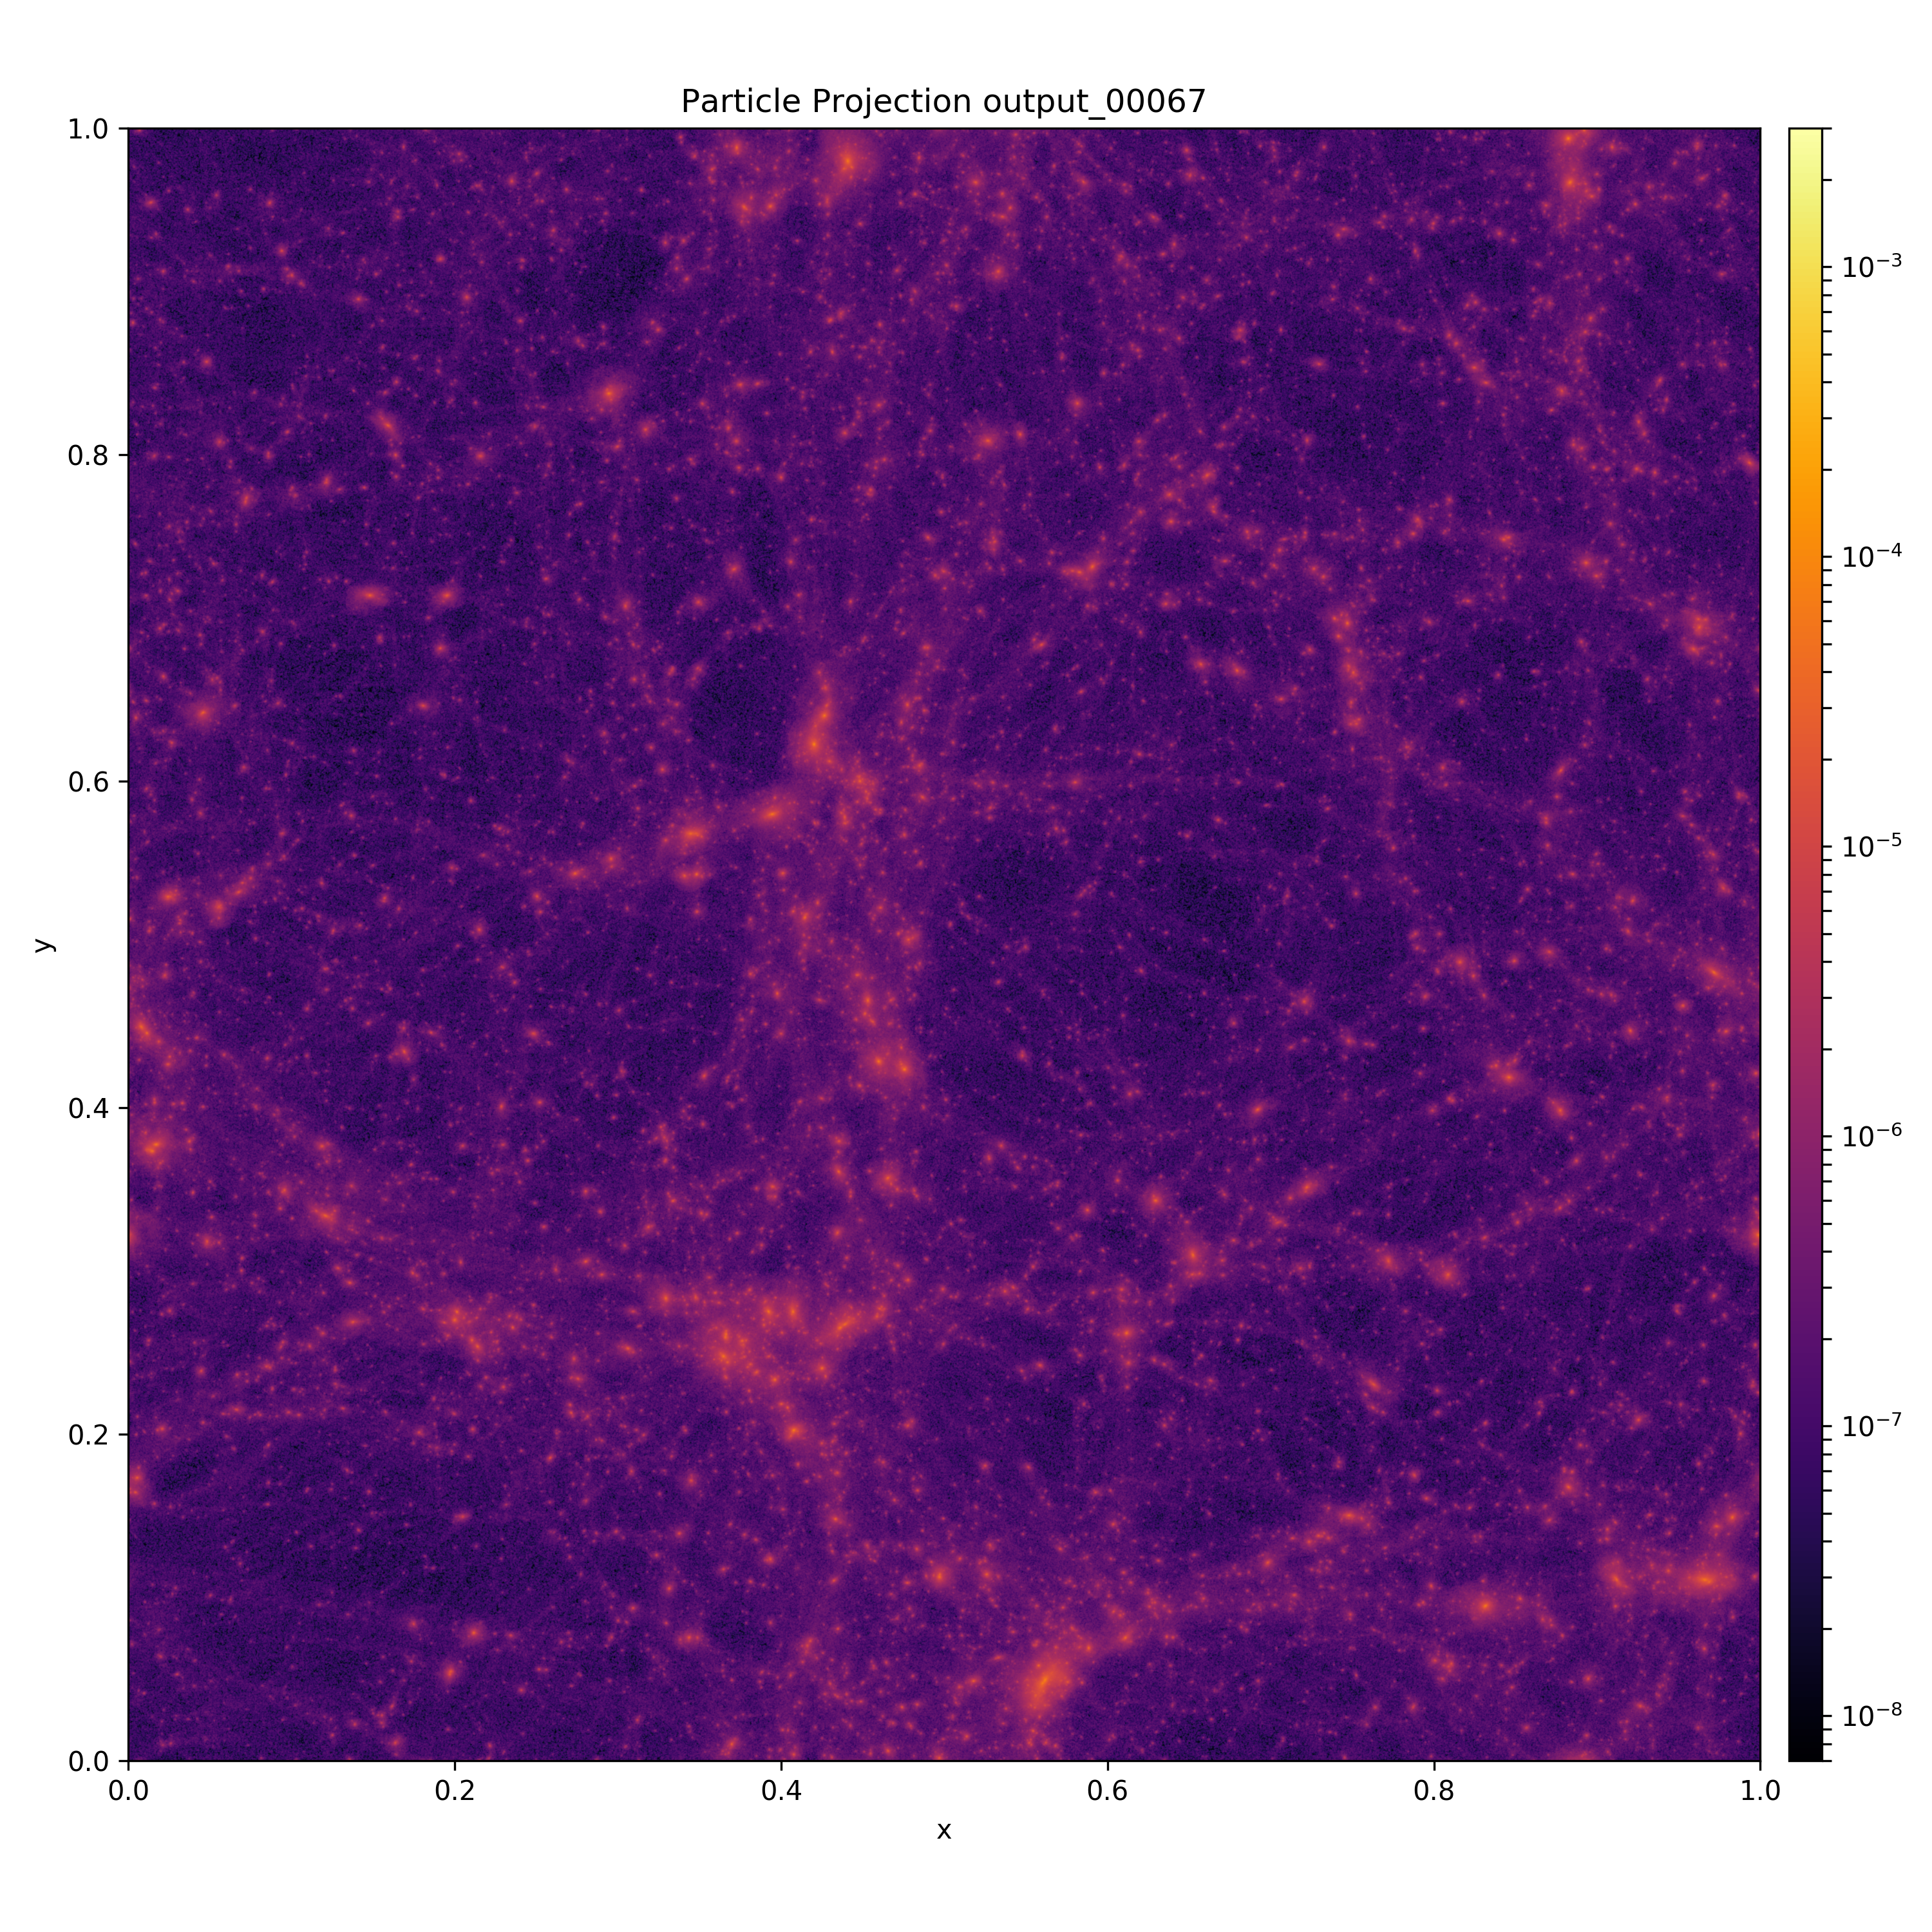
\includegraphics[keepaspectratio,height=\paperheight, width=\paperwidth]{./images/dm-vs-galaxies-256/particleplot_00067.png}\hfil}\vfil}}
    \begin{frame}[plain]
    \end{frame}
}

{
    \setbeamertemplate{background}
    {\vbox to \paperheight{\vfil \hbox to \paperwidth{\hfil\includegraphics[keepaspectratio,height=\paperheight, width=\paperwidth]{./images/dm-vs-galaxies-256/galaxy_density_projection-00067.png}\hfil}\vfil}}
    \begin{frame}[plain]
    \end{frame}
}

{
    \setbeamertemplate{background}
    {\vbox to \paperheight{\vfil \hbox to \paperwidth{\hfil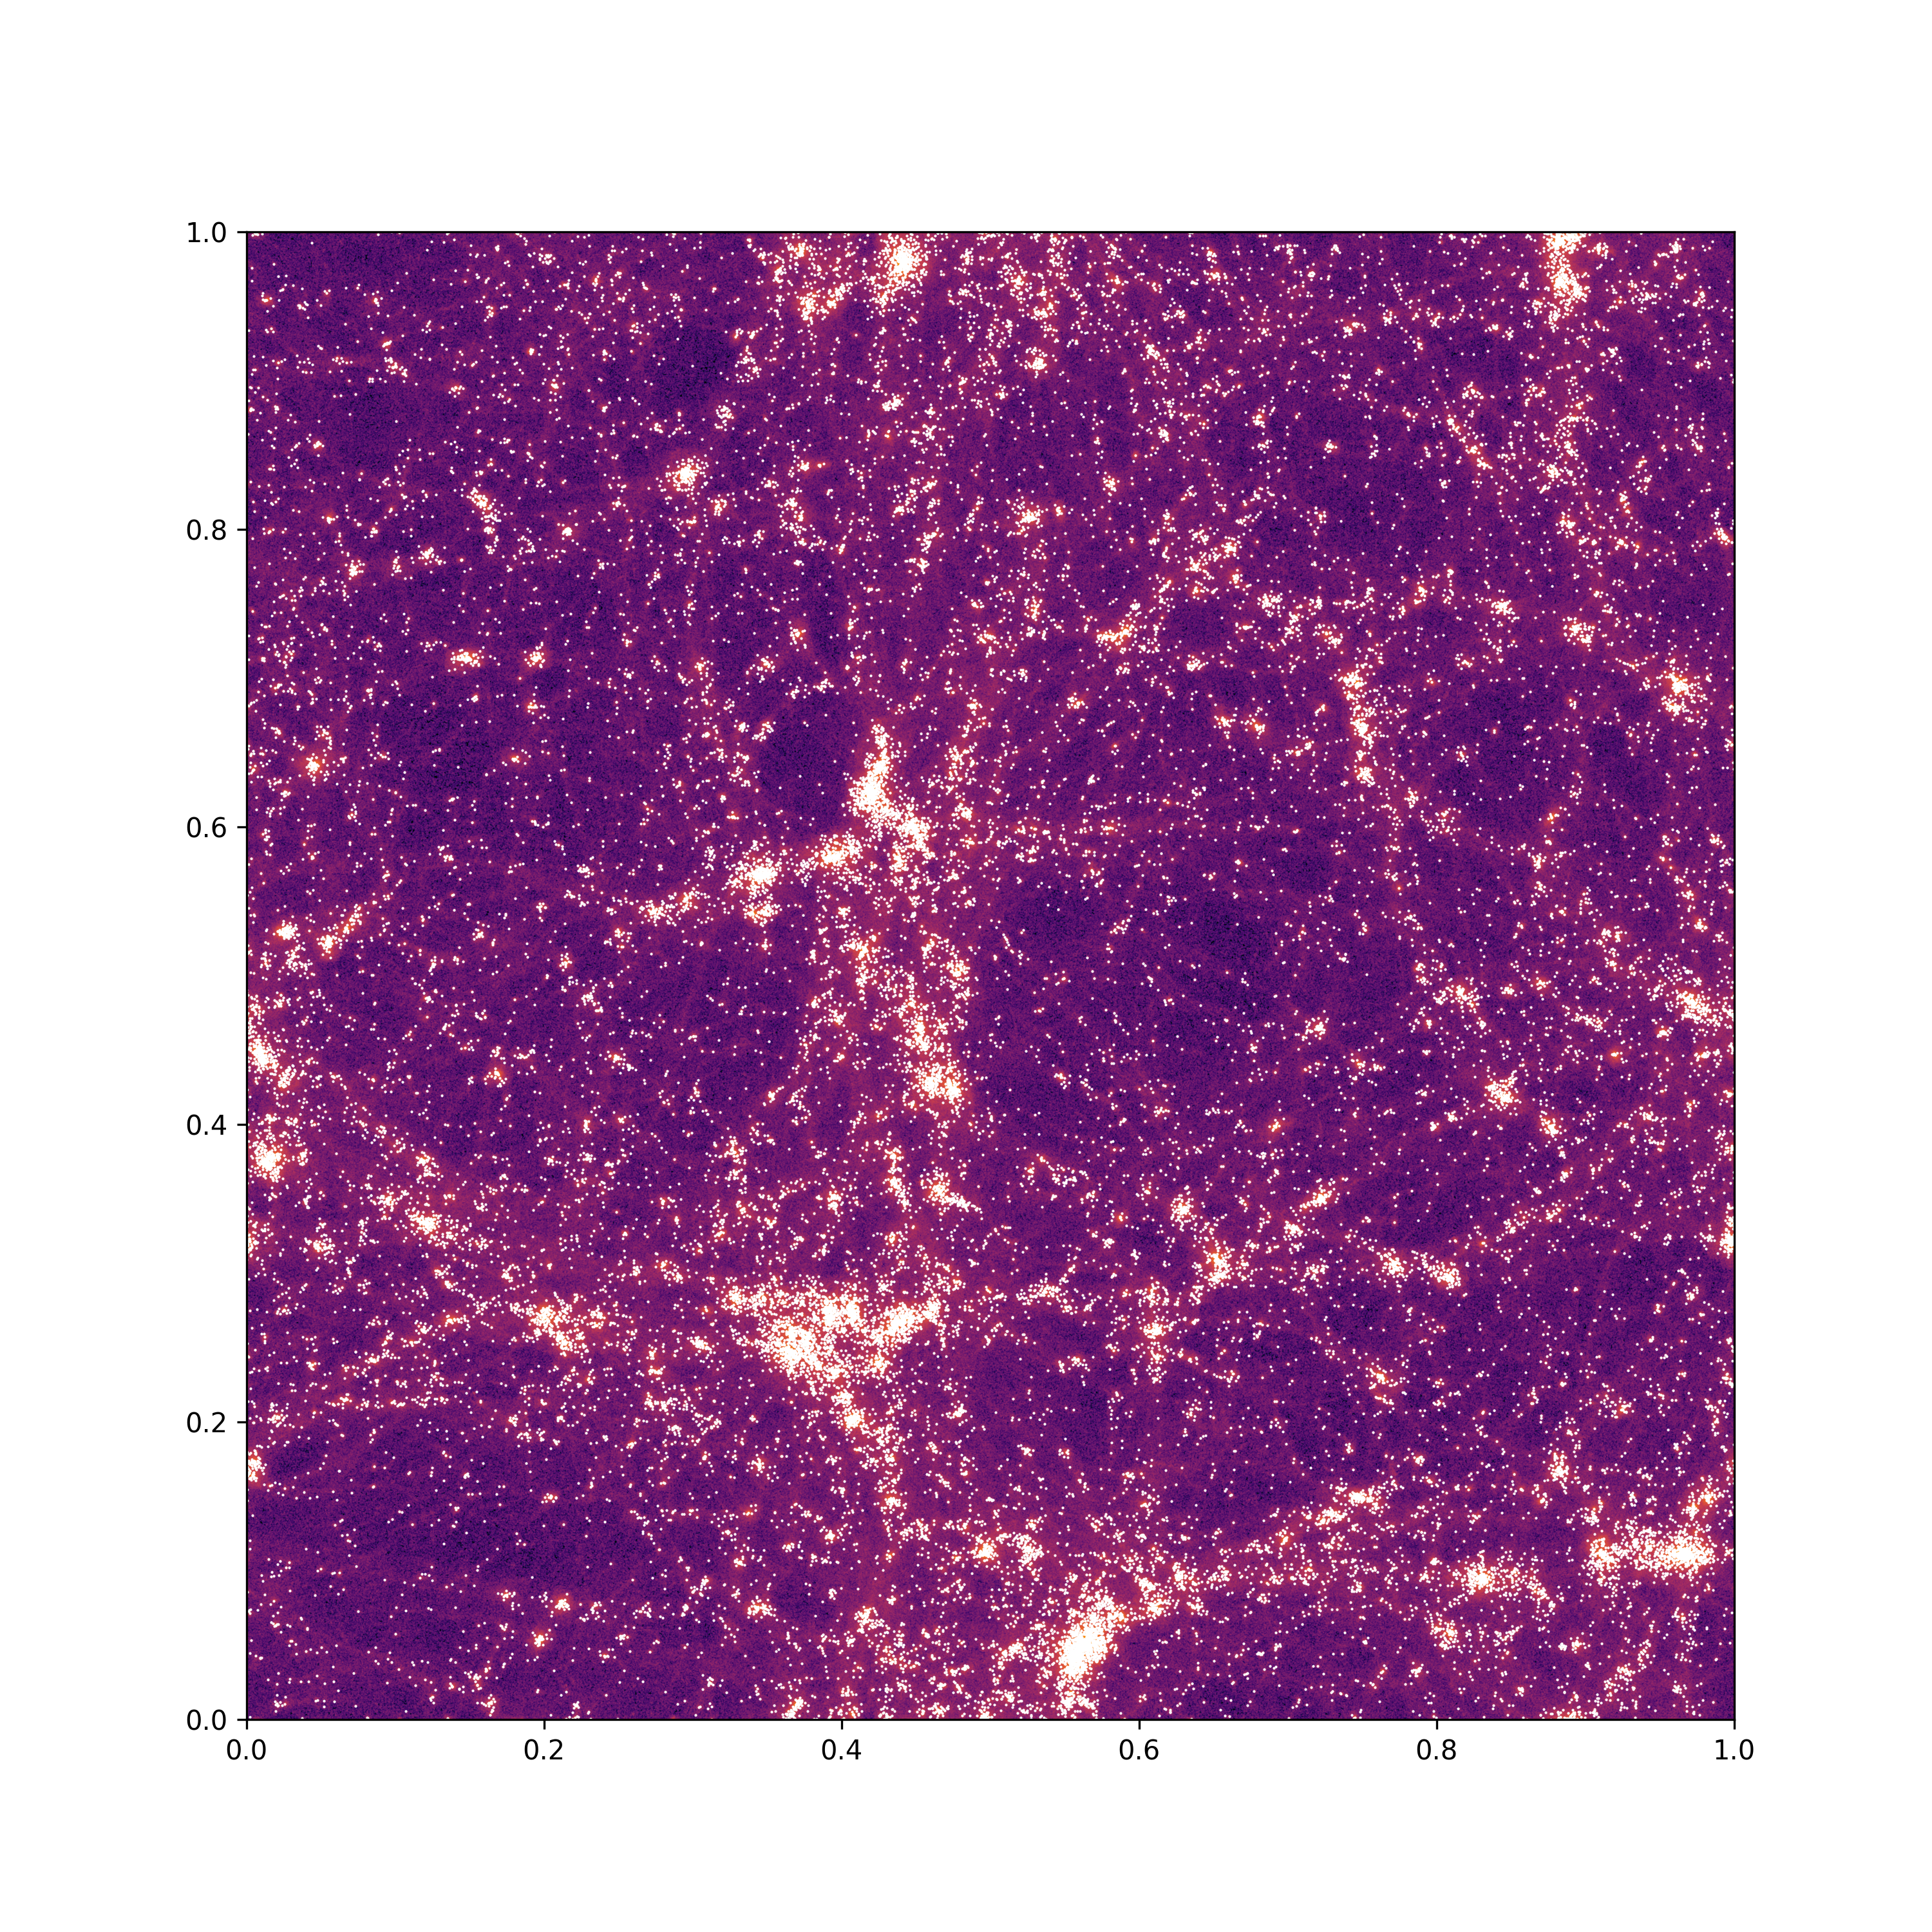
\includegraphics[keepaspectratio,height=\paperheight, width=\paperwidth]{./images/dm-vs-galaxies-256/galaxy_plot.png}\hfil}\vfil}}
    \begin{frame}[plain]
    \end{frame}
}

%\begin{frame}
%    
%\end{frame}
%
%
%
%{
%    \setbeamertemplate{background}
%    {\vbox to \paperheight{\vfil \hbox to \paperwidth{\hfil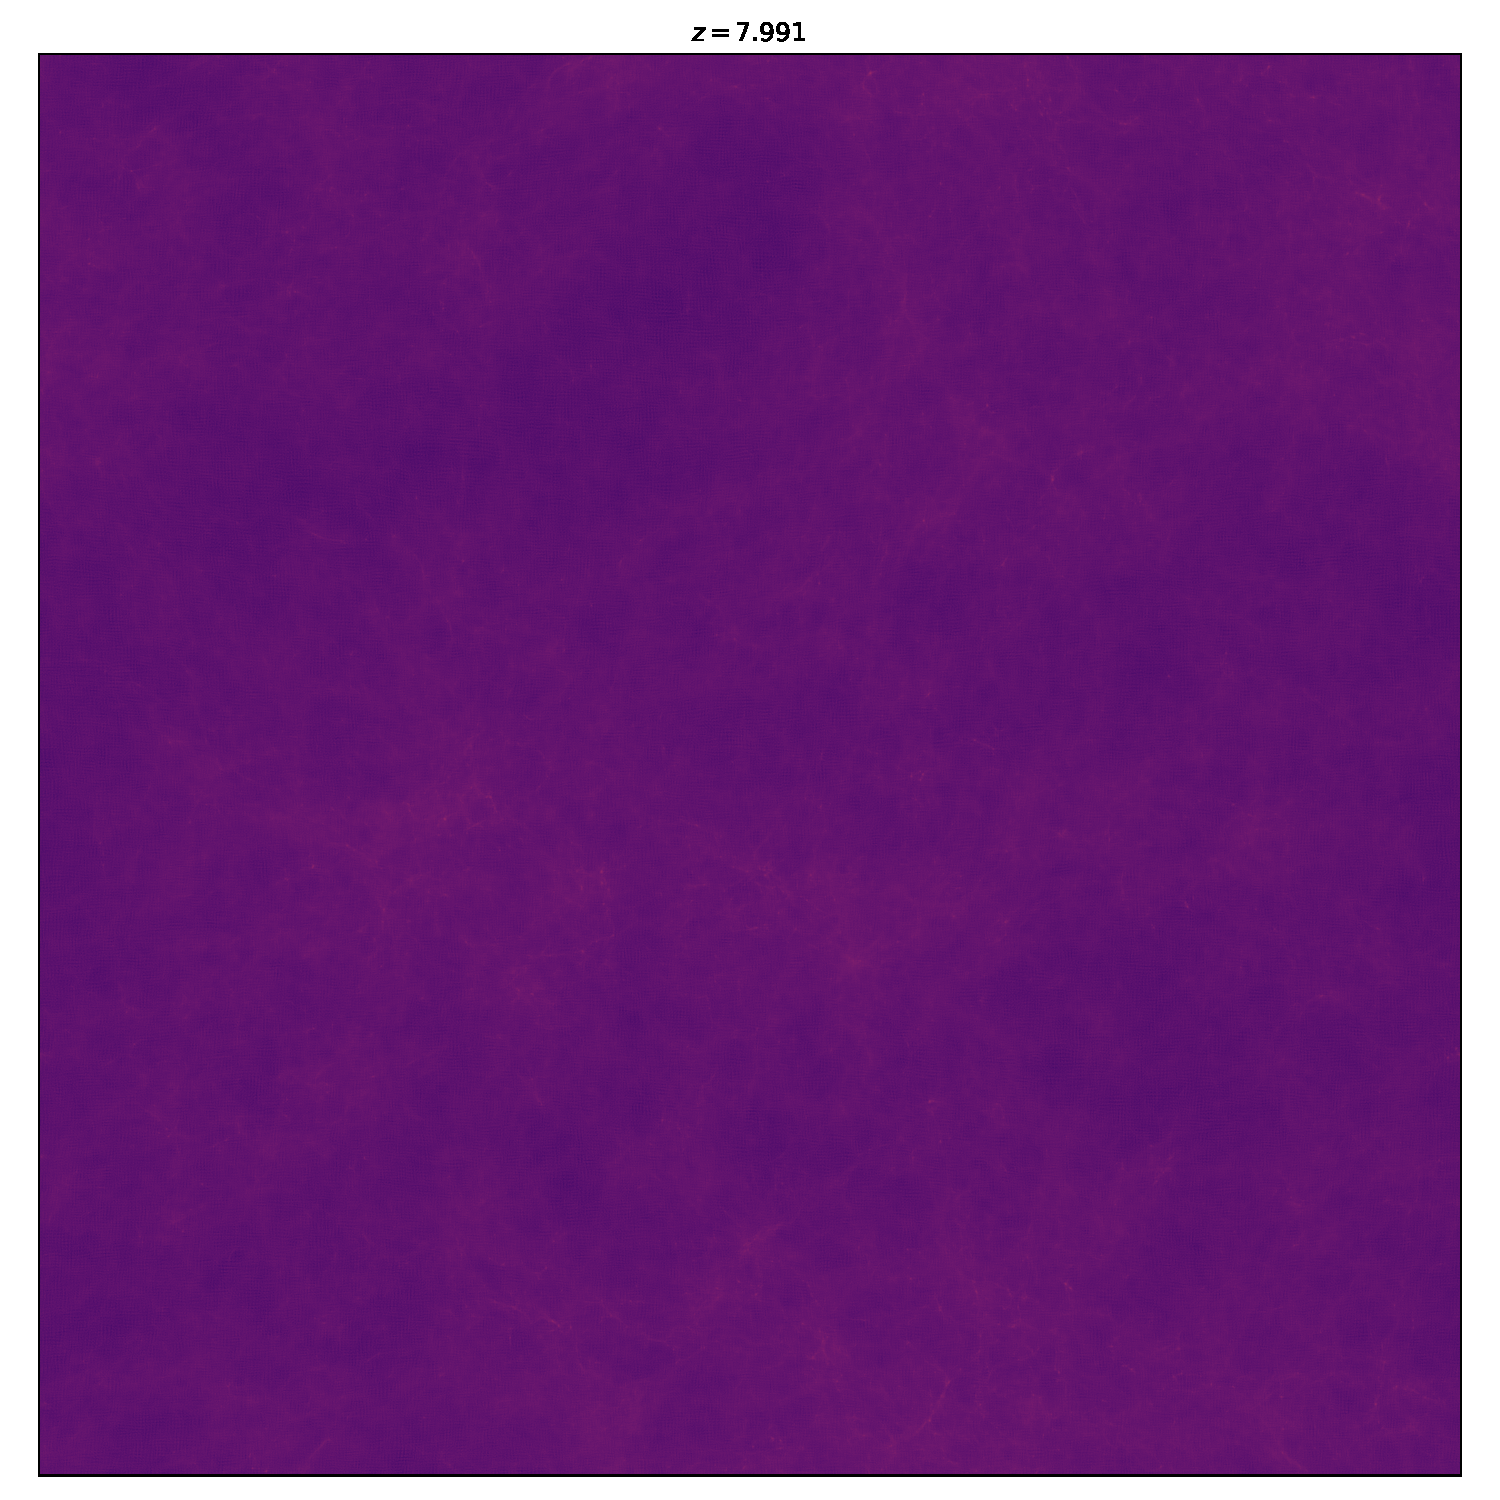
\includegraphics[keepaspectratio,height=\paperheight, width=\paperwidth]{./images/snapshots/particleplot_00002_nolabels.pdf}\hfil}\vfil}}
%    \begin{frame}[plain]
%    \end{frame}
%}
%{
%    \setbeamertemplate{background}
%    {\vbox to \paperheight{\vfil \hbox to \paperwidth{\hfil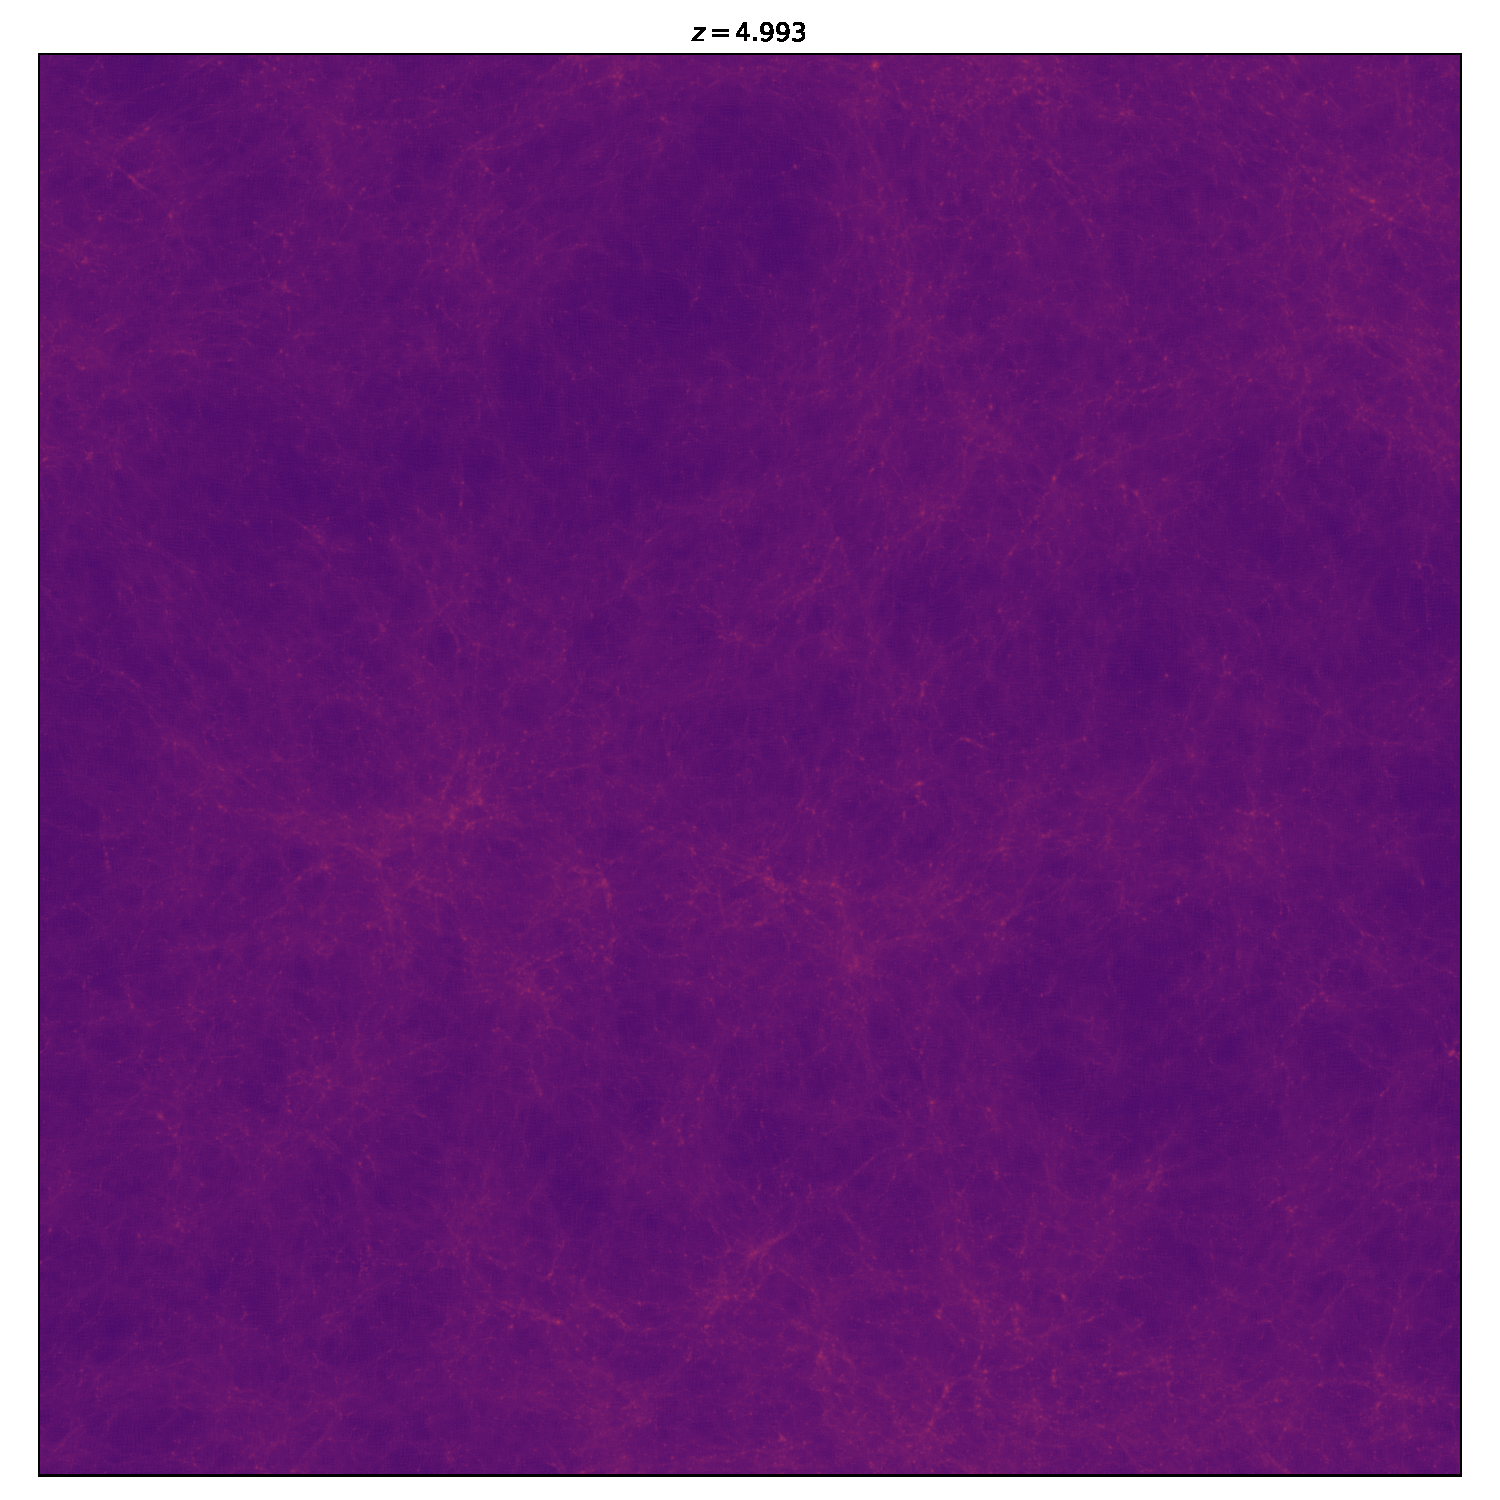
\includegraphics[keepaspectratio,height=\paperheight, width=\paperwidth]{./images/snapshots/particleplot_00005_nolabels.pdf}\hfil}\vfil}}
%    \begin{frame}[plain]
%    \end{frame}
%}
%{
%    \setbeamertemplate{background}
%    {\vbox to \paperheight{\vfil \hbox to \paperwidth{\hfil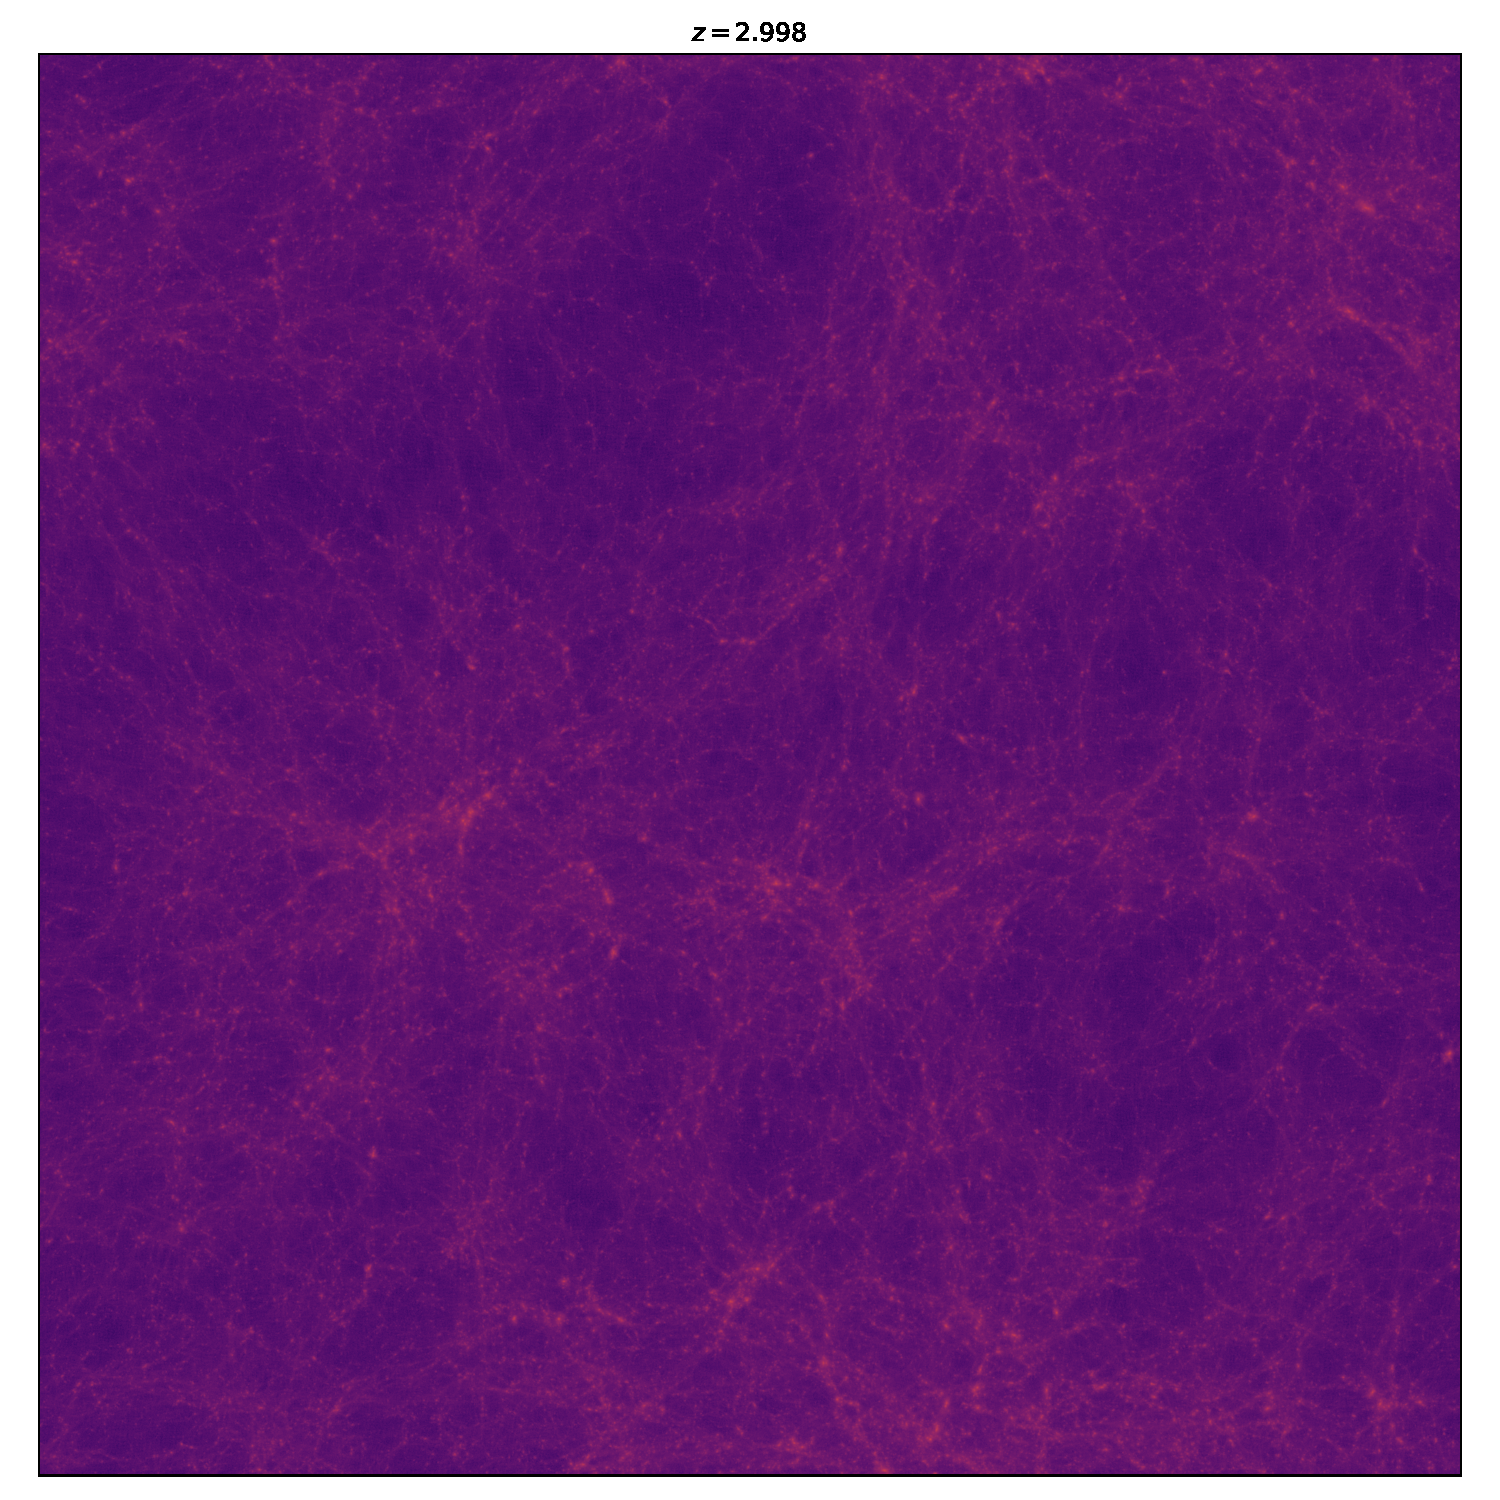
\includegraphics[keepaspectratio,height=\paperheight, width=\paperwidth]{./images/snapshots/particleplot_00008_nolabels.pdf}\hfil}\vfil}}
%    \begin{frame}[plain]
%    \end{frame}
%}
%{
%    \setbeamertemplate{background}
%    {\vbox to \paperheight{\vfil \hbox to \paperwidth{\hfil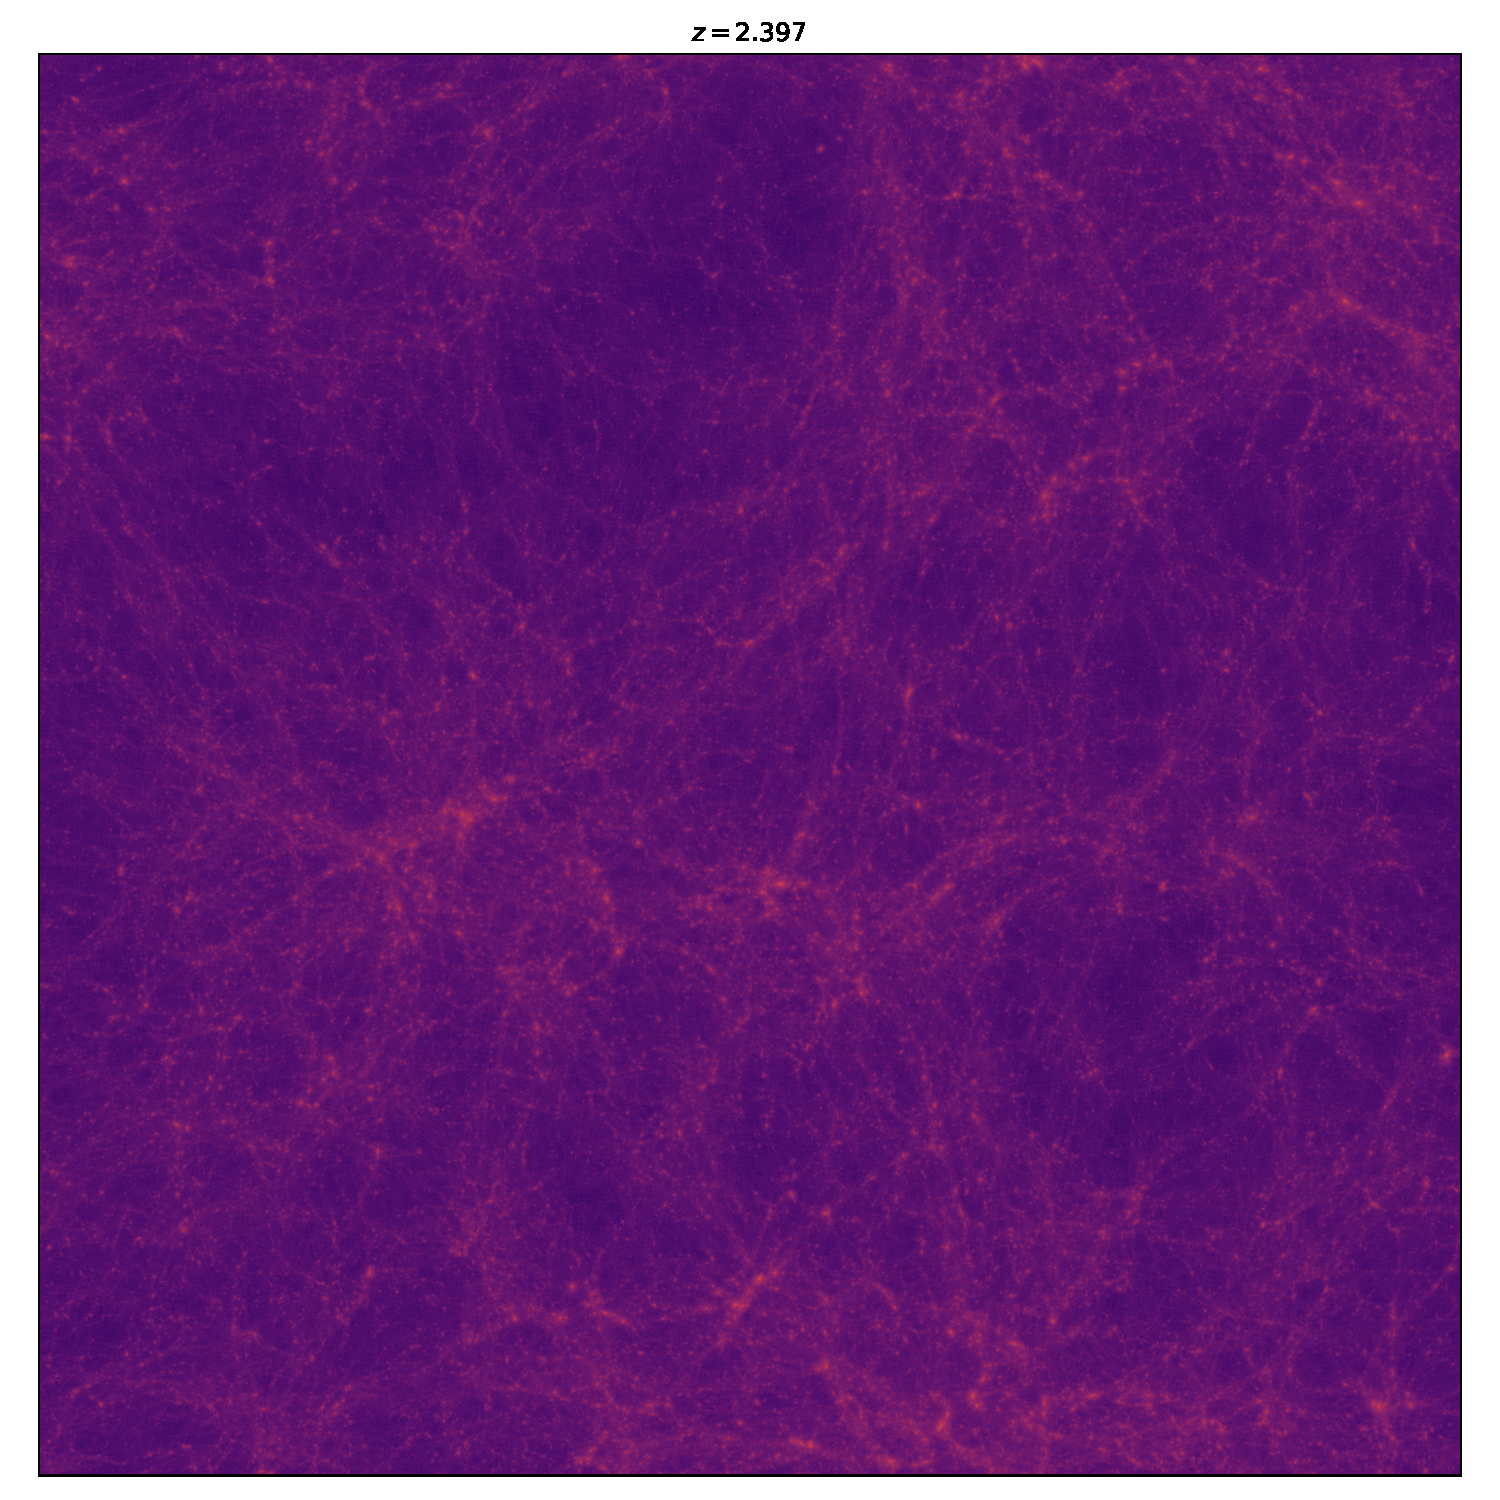
\includegraphics[keepaspectratio,height=\paperheight, width=\paperwidth]{./images/snapshots/particleplot_00011_nolabels.pdf}\hfil}\vfil}}
%    \begin{frame}[plain]
%    \end{frame}
%}
%{
%    \setbeamertemplate{background}
%    {\vbox to \paperheight{\vfil \hbox to \paperwidth{\hfil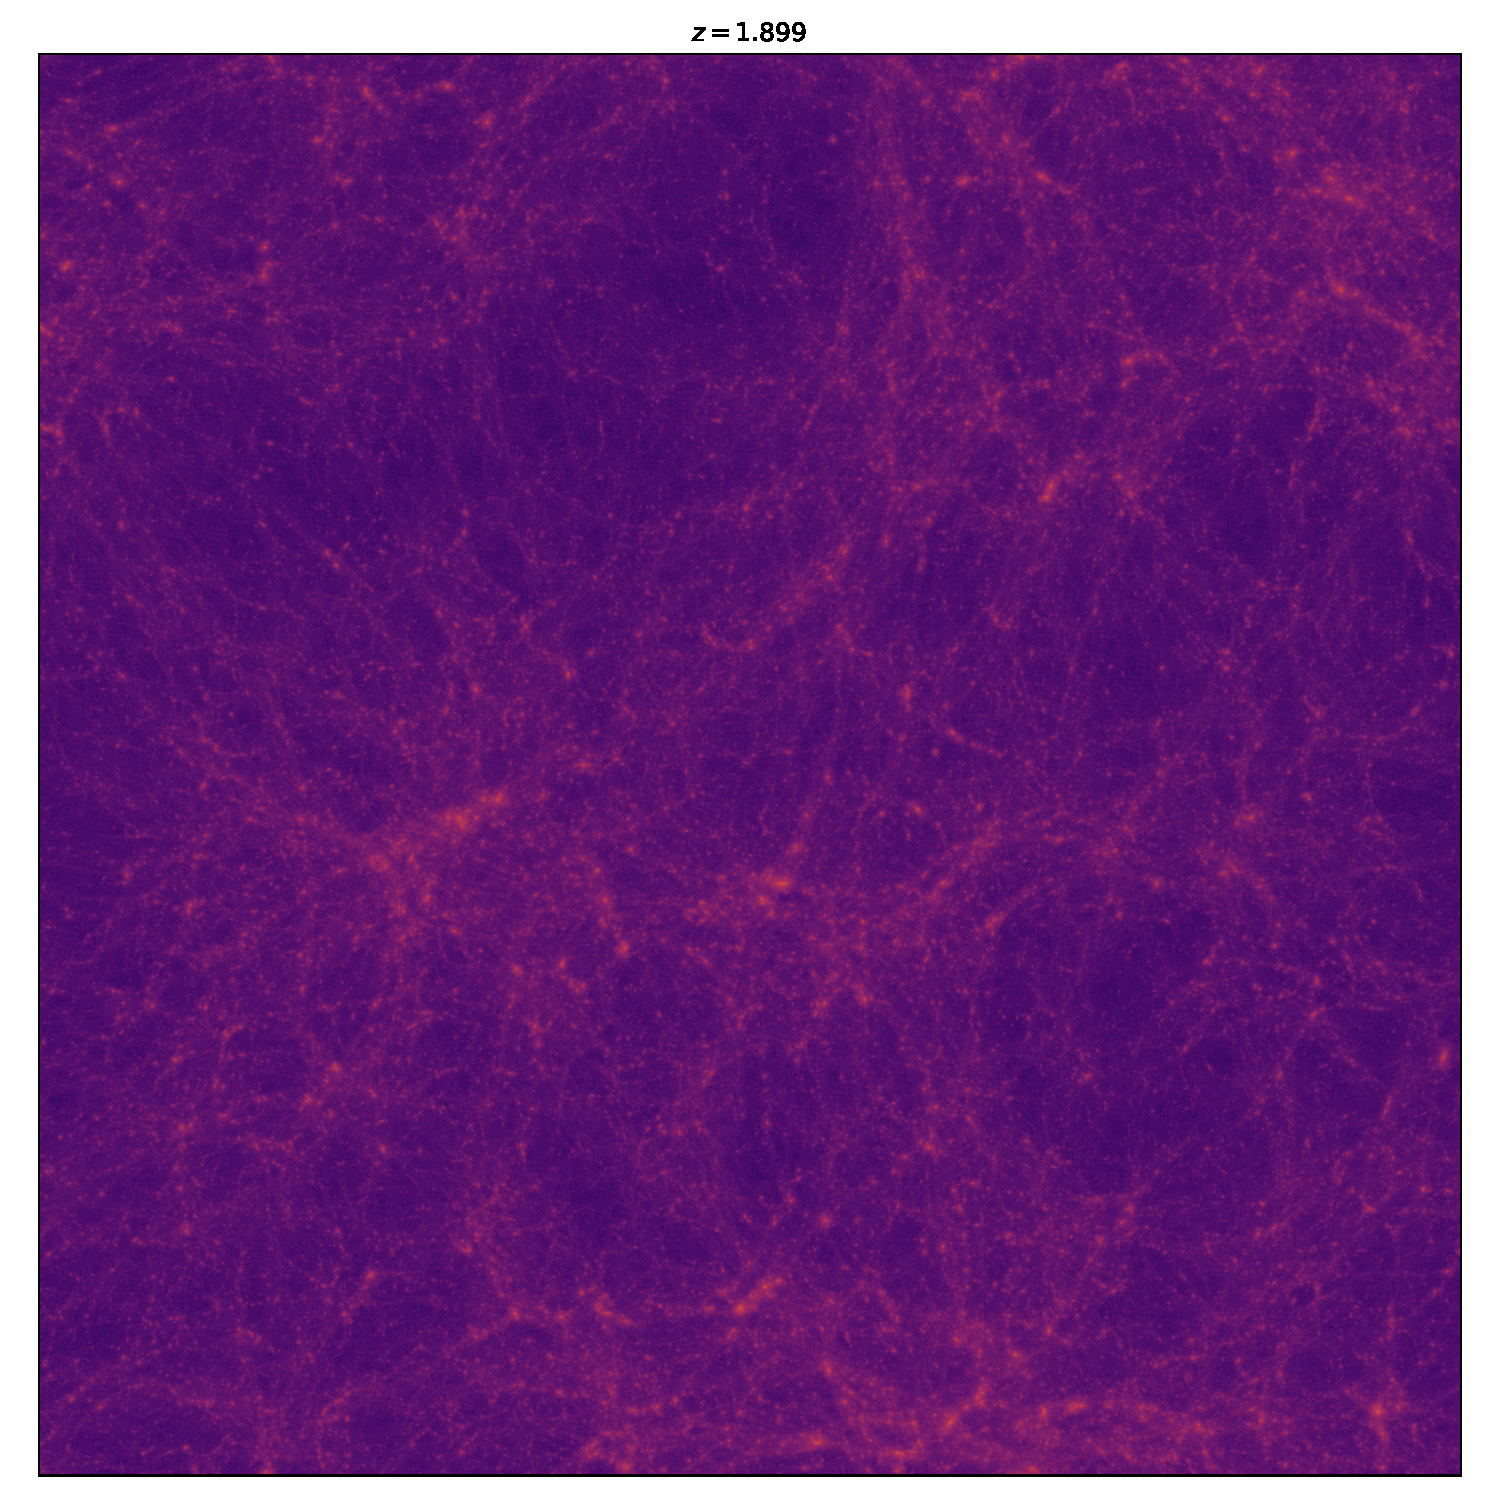
\includegraphics[keepaspectratio,height=\paperheight, width=\paperwidth]{./images/snapshots/particleplot_00014_nolabels.pdf}\hfil}\vfil}}
%    \begin{frame}[plain]
%    \end{frame}
%}
%{
%    \setbeamertemplate{background}
%    {\vbox to \paperheight{\vfil \hbox to \paperwidth{\hfil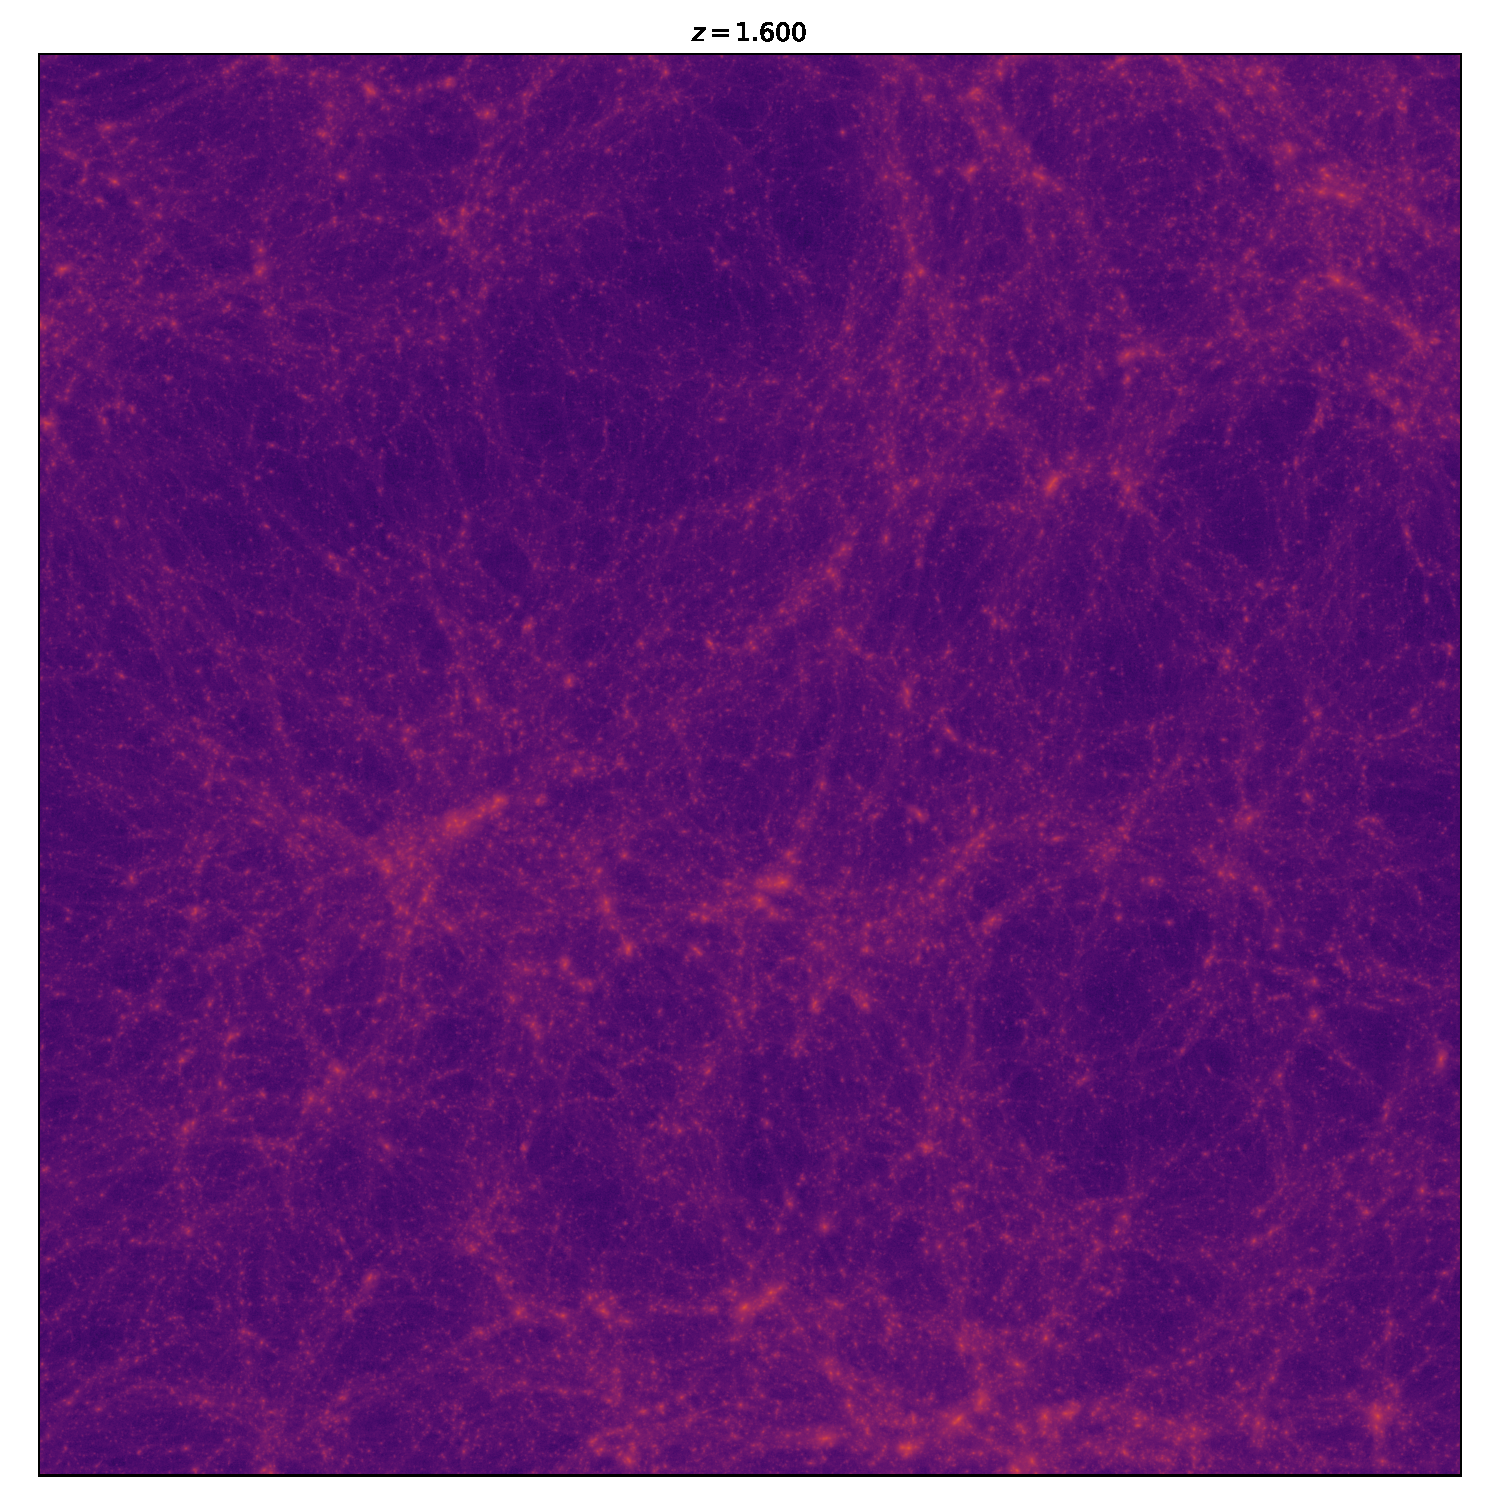
\includegraphics[keepaspectratio,height=\paperheight, width=\paperwidth]{./images/snapshots/particleplot_00017_nolabels.pdf}\hfil}\vfil}}
%    \begin{frame}[plain]
%    \end{frame}
%}
%{
%    \setbeamertemplate{background}
%    {\vbox to \paperheight{\vfil \hbox to \paperwidth{\hfil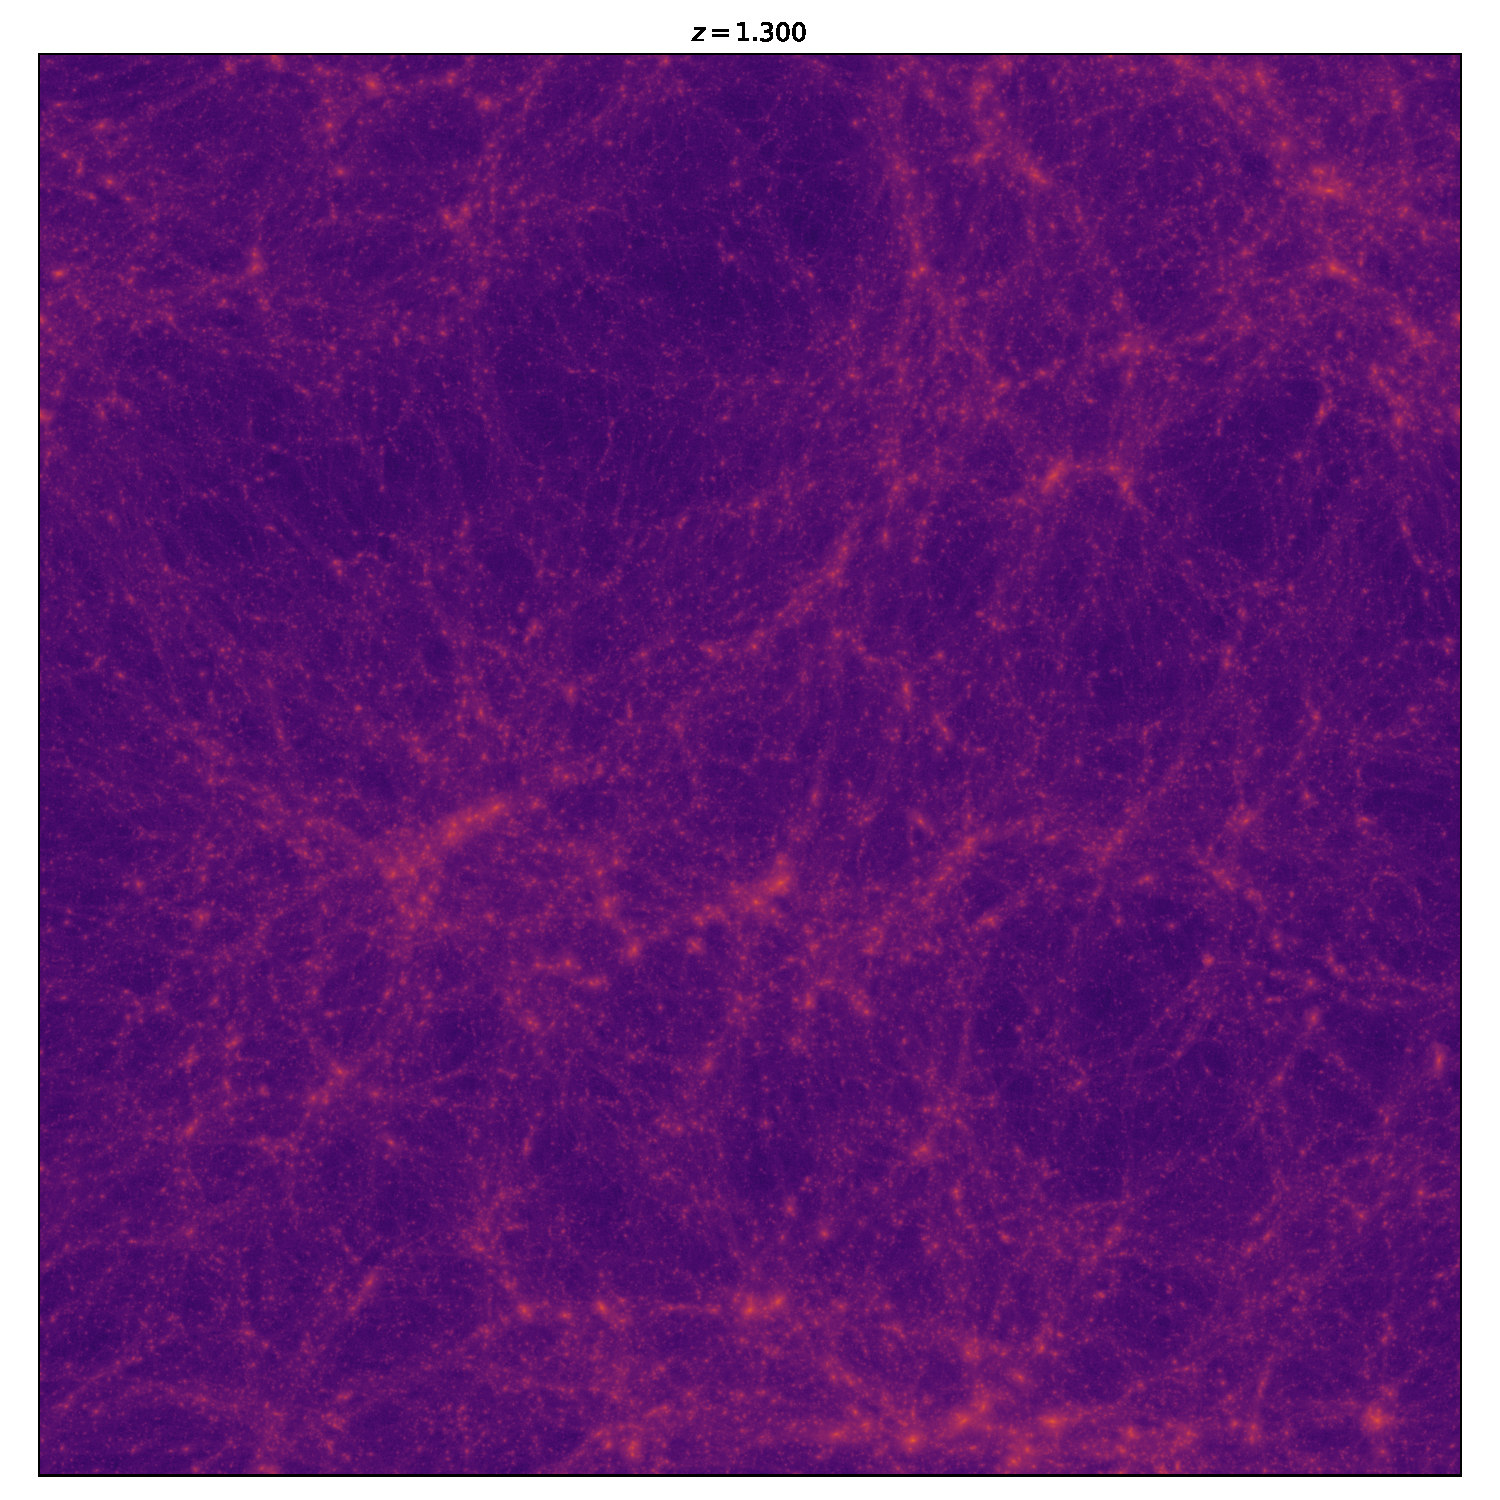
\includegraphics[keepaspectratio,height=\paperheight, width=\paperwidth]{./images/snapshots/particleplot_00020_nolabels.pdf}\hfil}\vfil}}
%    \begin{frame}[plain]
%    \end{frame}
%}
%{
%    \setbeamertemplate{background}
%    {\vbox to \paperheight{\vfil \hbox to \paperwidth{\hfil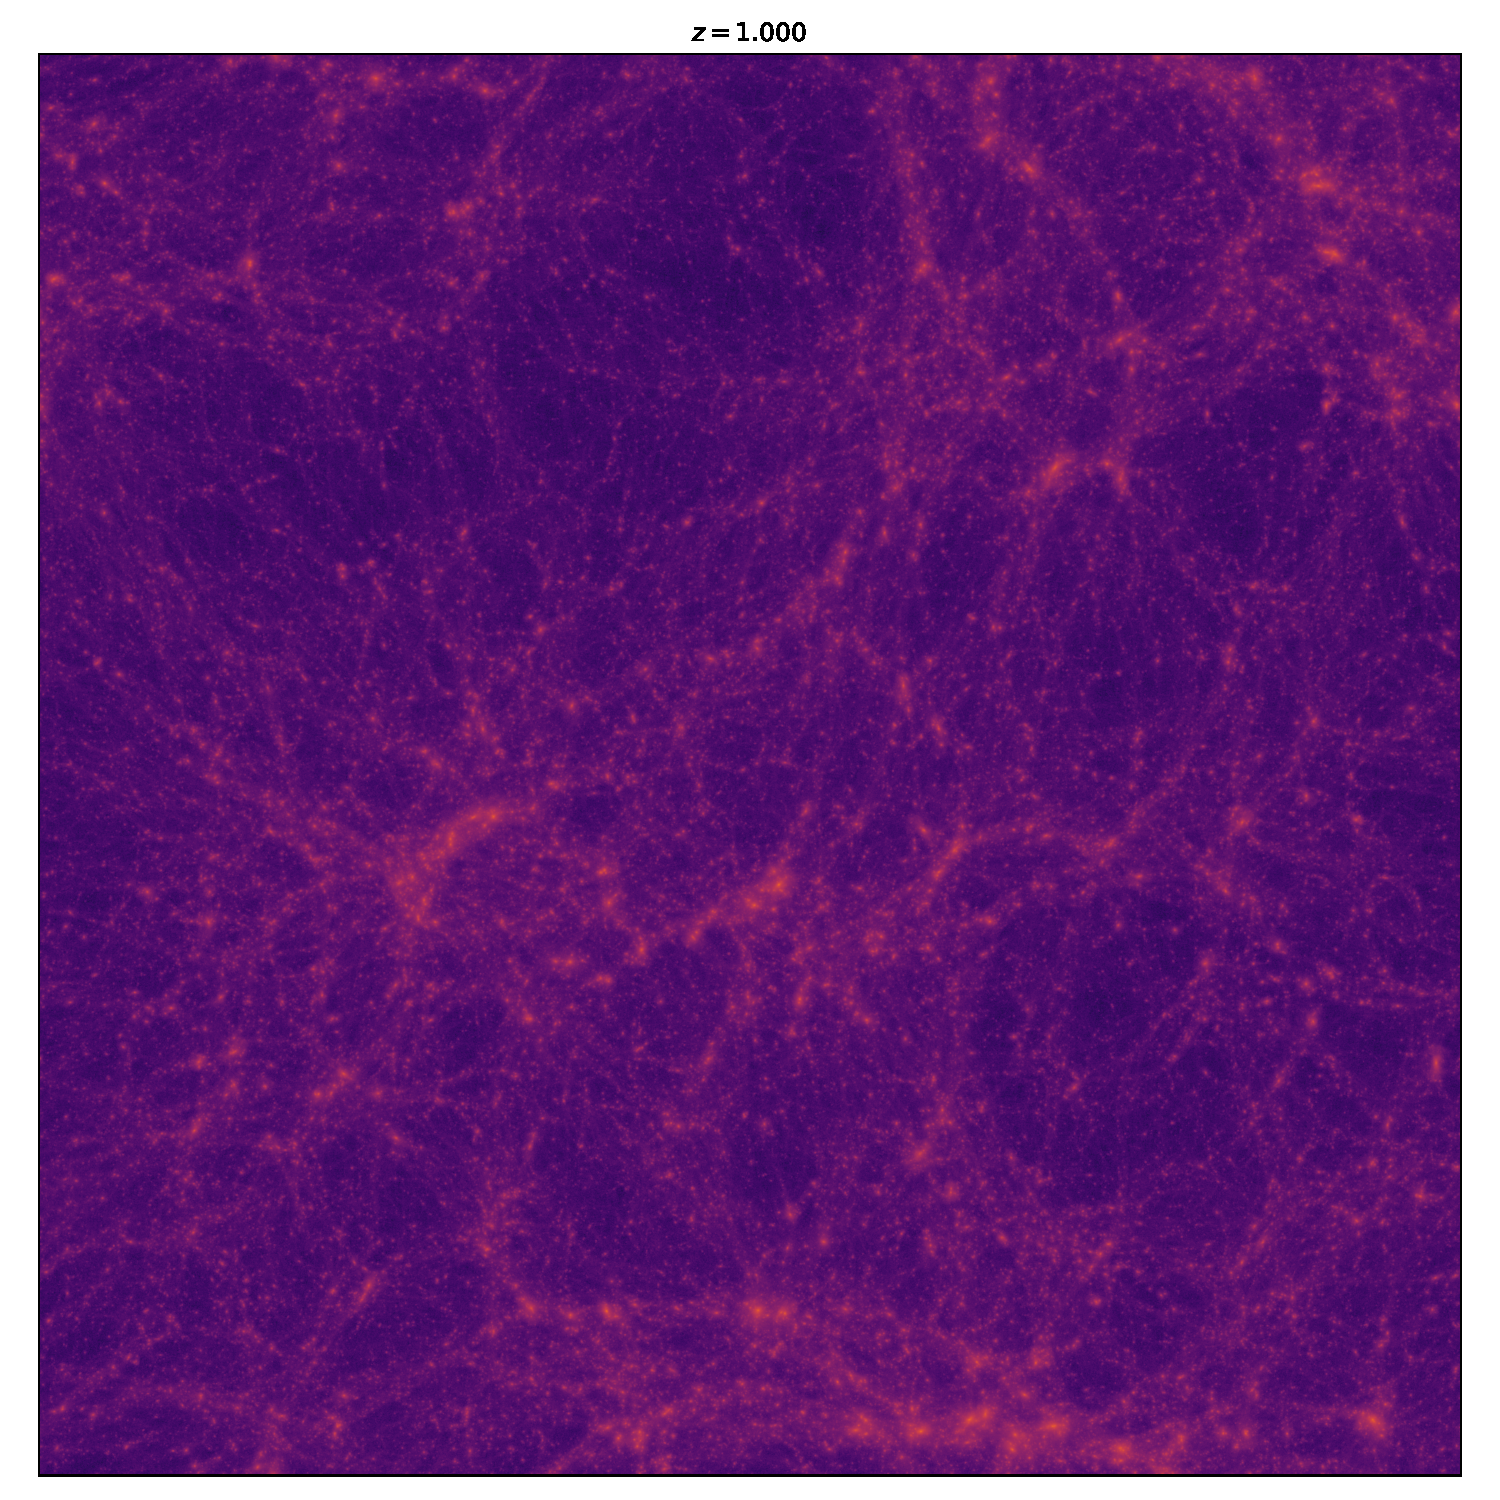
\includegraphics[keepaspectratio,height=\paperheight, width=\paperwidth]{./images/snapshots/particleplot_00023_nolabels.pdf}\hfil}\vfil}}
%    \begin{frame}[plain]
%    \end{frame}
%}
%{
%    \setbeamertemplate{background}
%    {\vbox to \paperheight{\vfil \hbox to \paperwidth{\hfil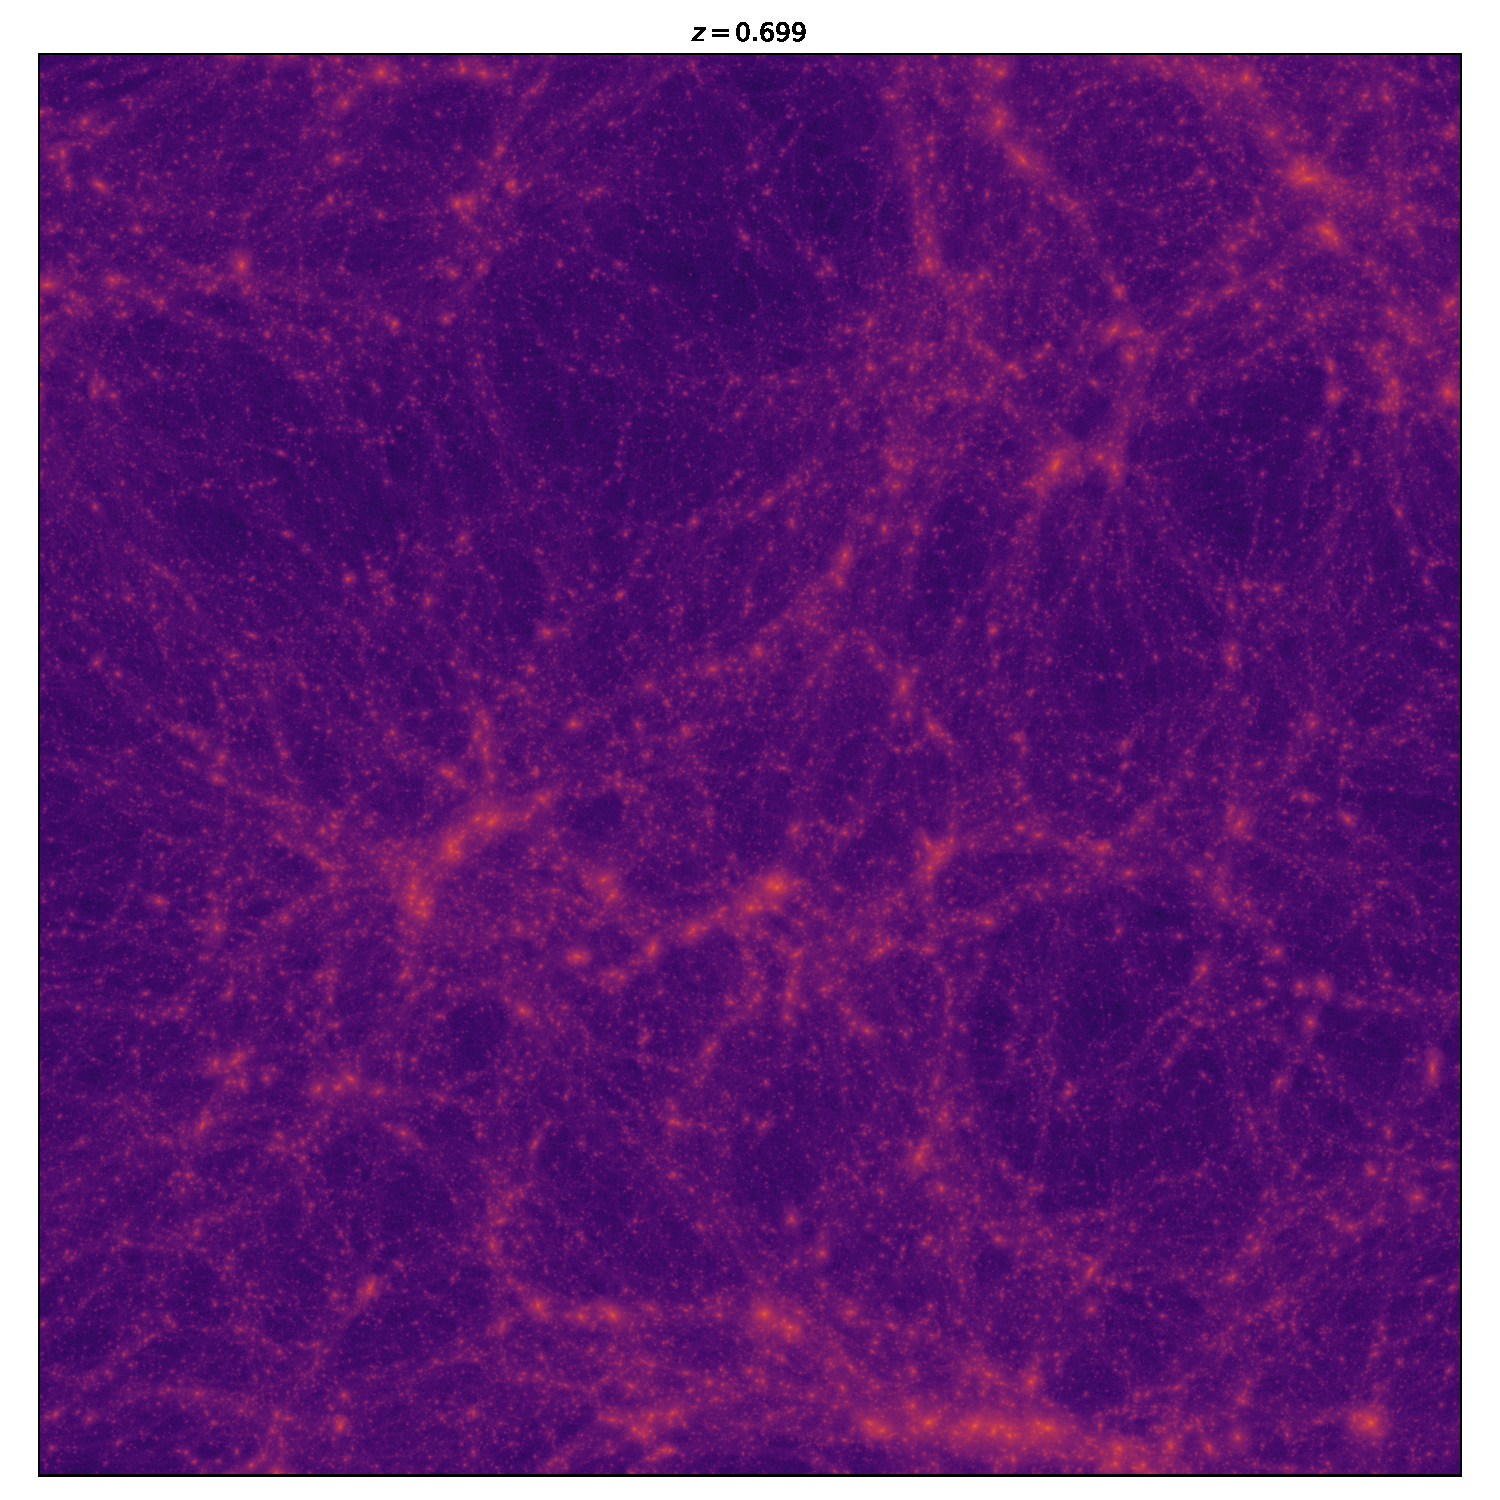
\includegraphics[keepaspectratio,height=\paperheight, width=\paperwidth]{./images/snapshots/particleplot_00026_nolabels.pdf}\hfil}\vfil}}
%    \begin{frame}[plain]
%    \end{frame}
%}
%{
%    \setbeamertemplate{background}
%    {\vbox to \paperheight{\vfil \hbox to \paperwidth{\hfil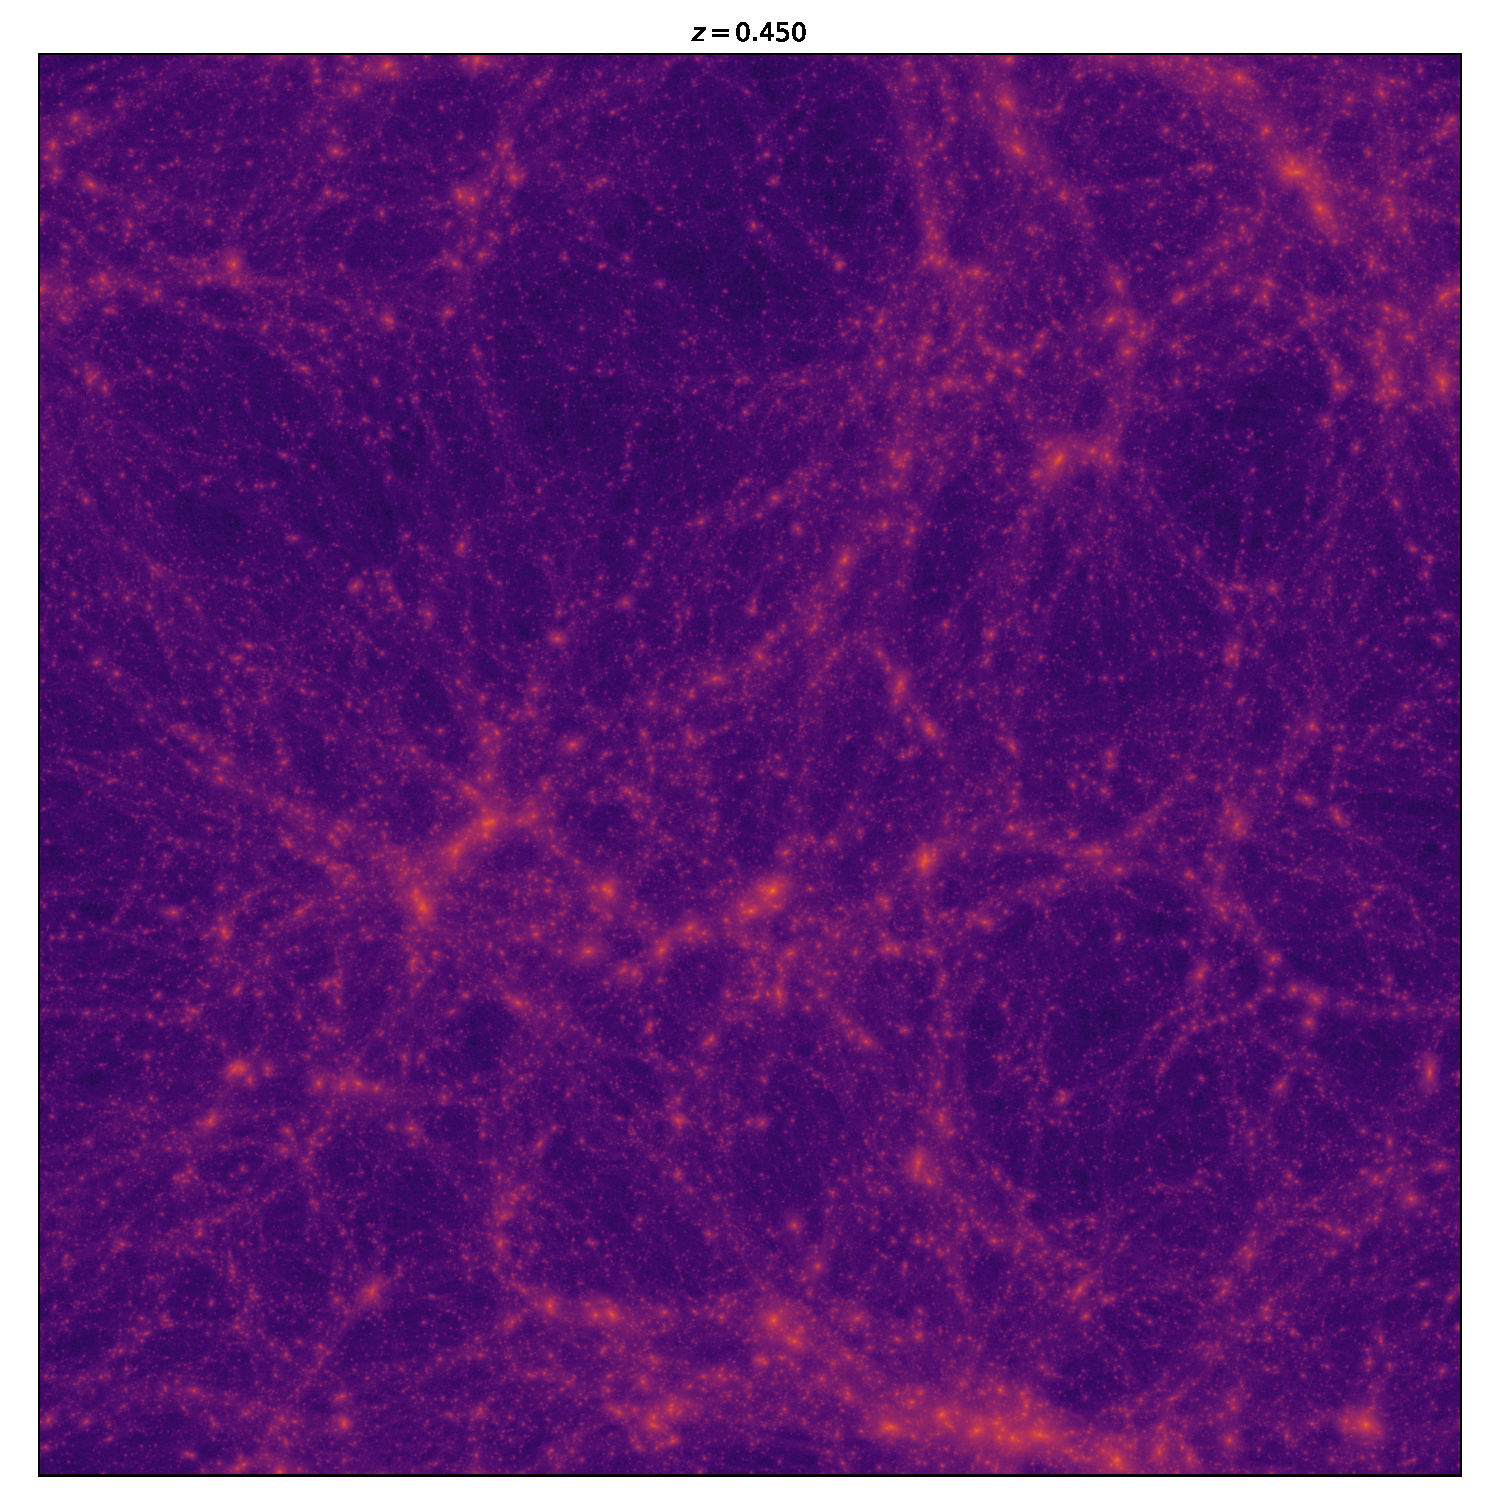
\includegraphics[keepaspectratio,height=\paperheight, width=\paperwidth]{./images/snapshots/particleplot_00029_nolabels.pdf}\hfil}\vfil}}
%    \begin{frame}[plain]
%    \end{frame}
%}
%{
%    \setbeamertemplate{background}
%    {\vbox to \paperheight{\vfil \hbox to \paperwidth{\hfil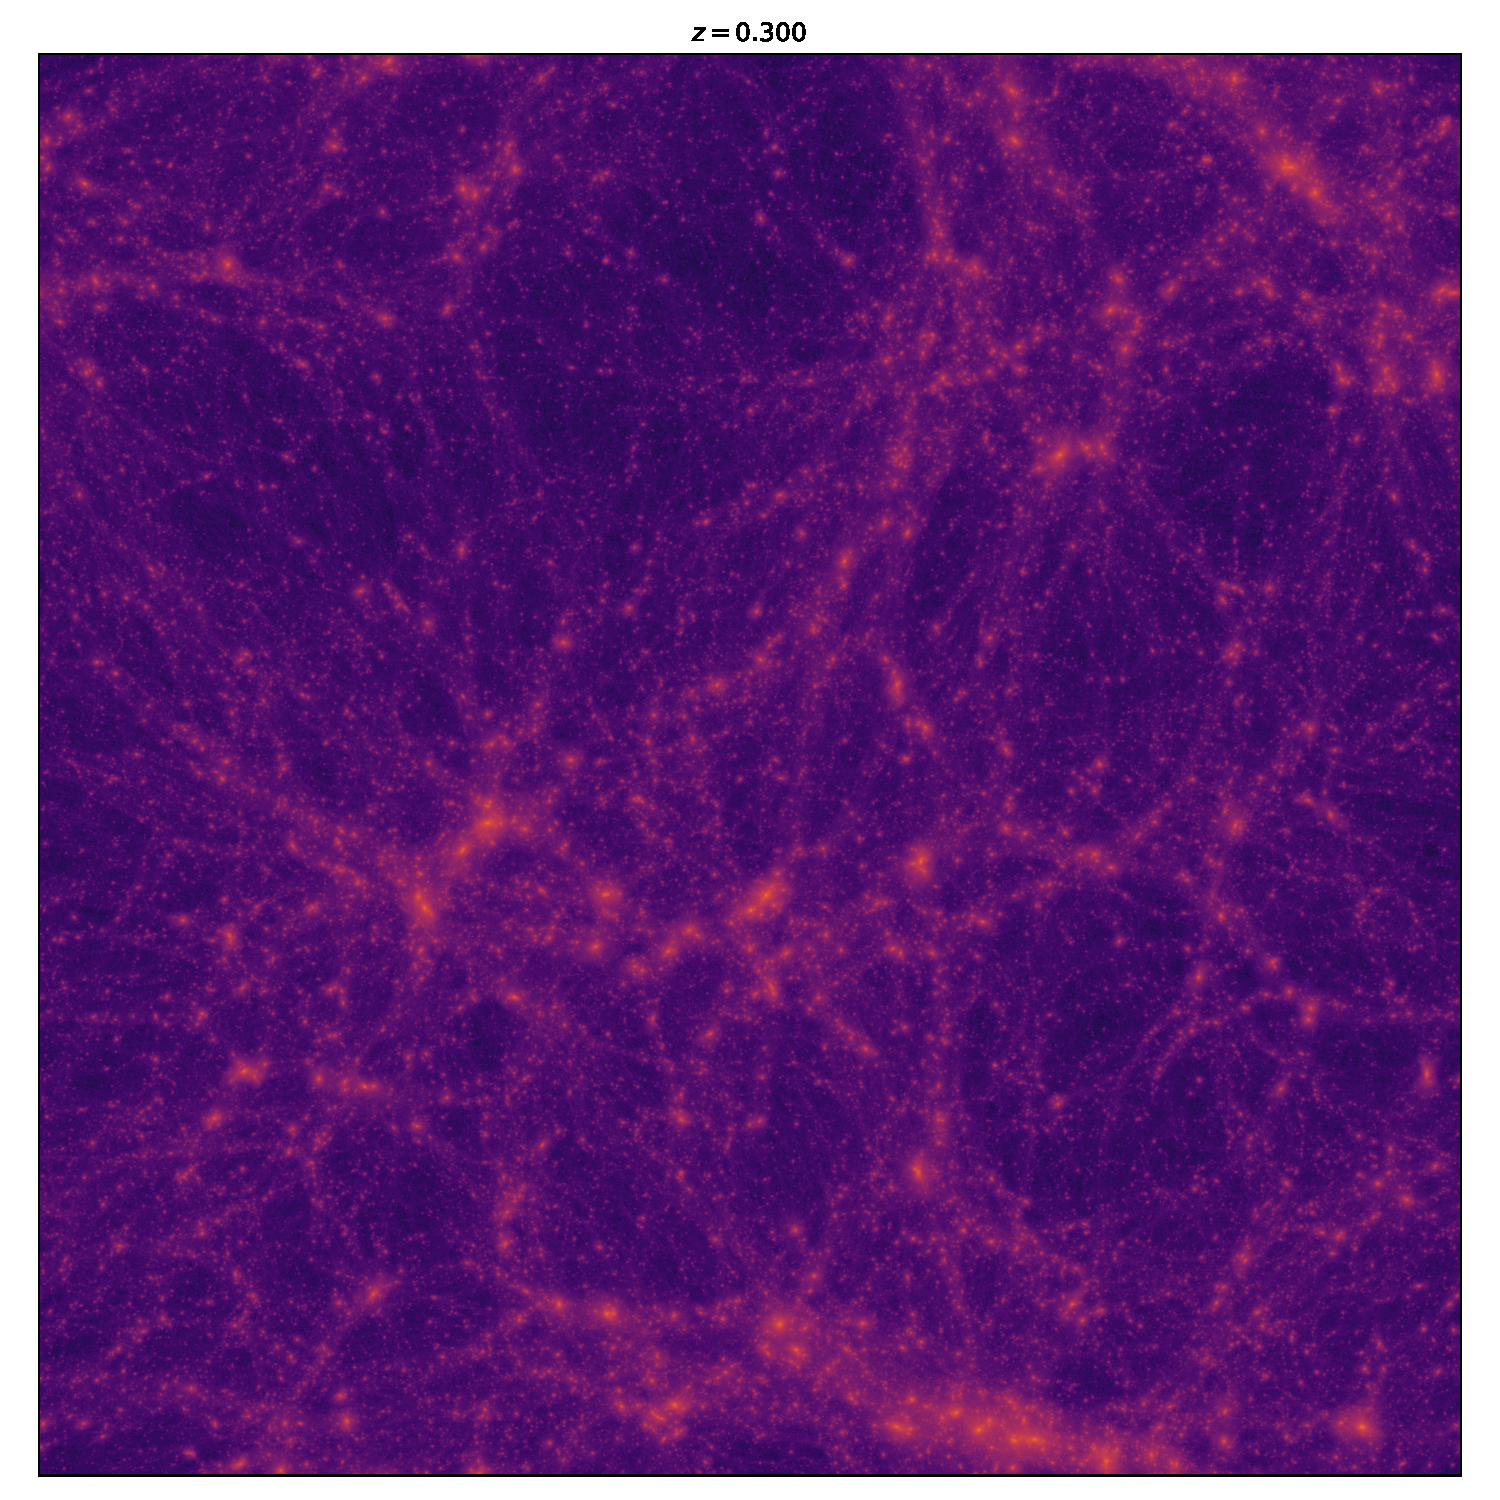
\includegraphics[keepaspectratio,height=\paperheight, width=\paperwidth]{./images/snapshots/particleplot_00032_nolabels.pdf}\hfil}\vfil}}
%    \begin{frame}[plain]
%    \end{frame}
%}
%{
%    \setbeamertemplate{background}
%    {\vbox to \paperheight{\vfil \hbox to \paperwidth{\hfil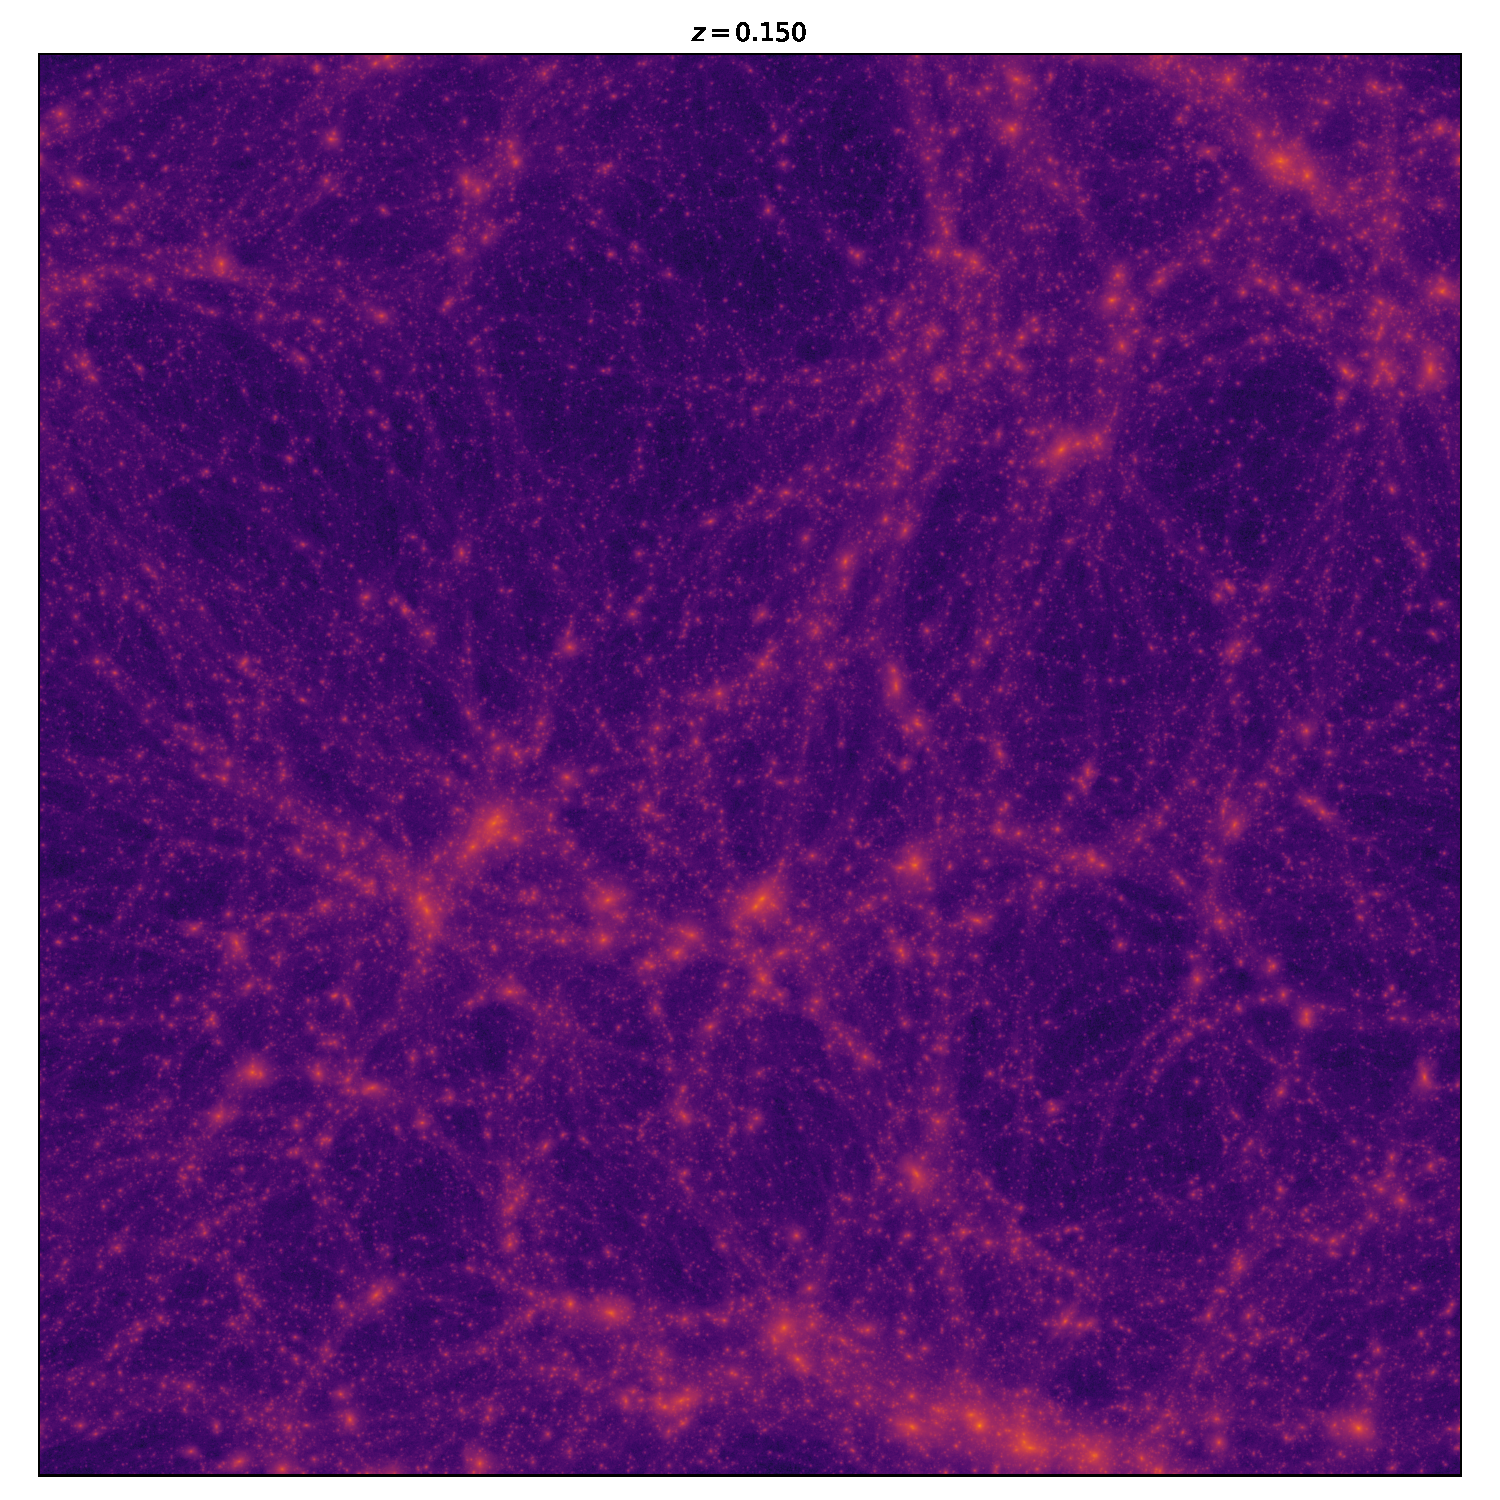
\includegraphics[keepaspectratio,height=\paperheight, width=\paperwidth]{./images/snapshots/particleplot_00035_nolabels.pdf}\hfil}\vfil}}
%    \begin{frame}[plain]
%    \end{frame}
%}
%{
%    \setbeamertemplate{background}
%    {\vbox to \paperheight{\vfil \hbox to \paperwidth{\hfil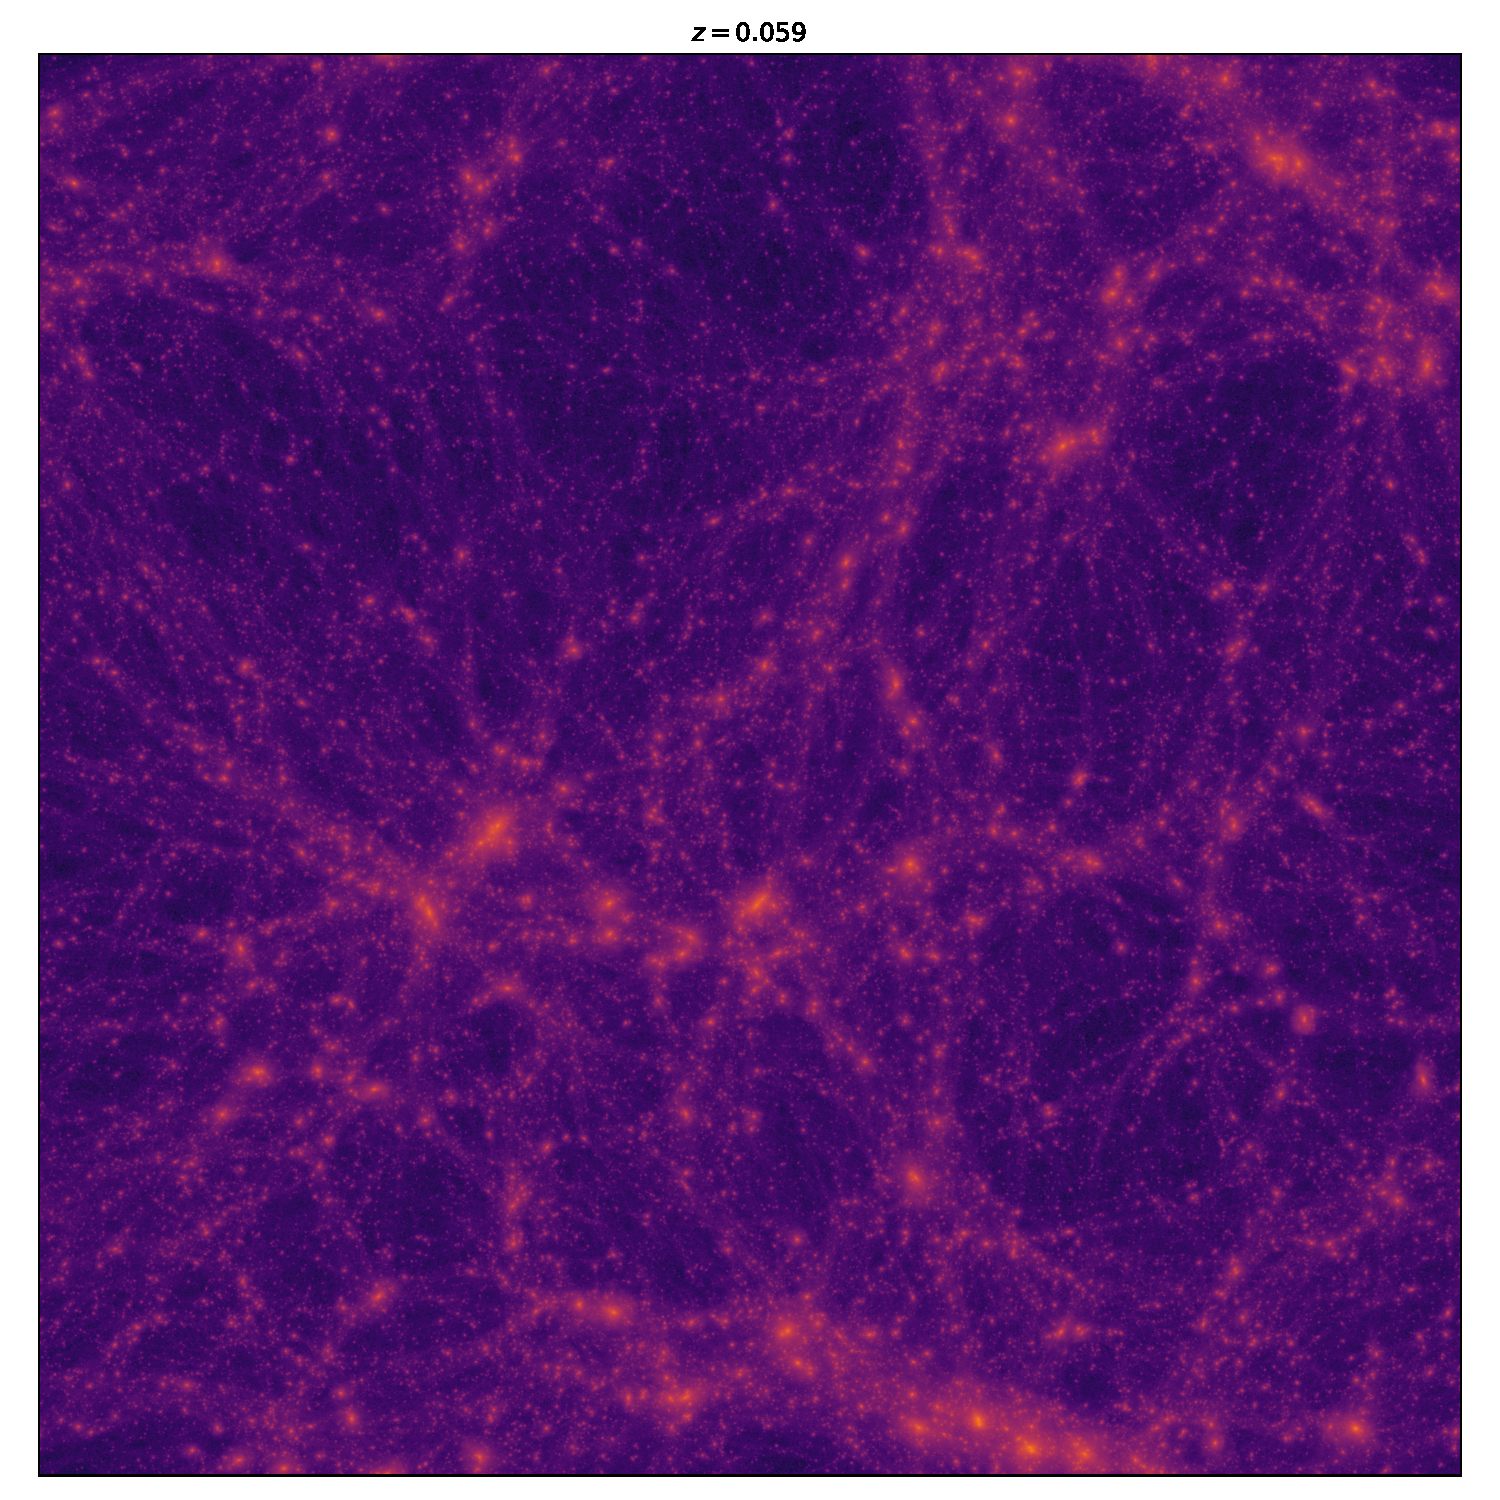
\includegraphics[keepaspectratio,height=\paperheight, width=\paperwidth]{./images/snapshots/particleplot_00038_nolabels.pdf}\hfil}\vfil}}
%    \begin{frame}[plain]
%    \end{frame}
%}
%{
%    \setbeamertemplate{background}
%    {\vbox to \paperheight{\vfil \hbox to \paperwidth{\hfil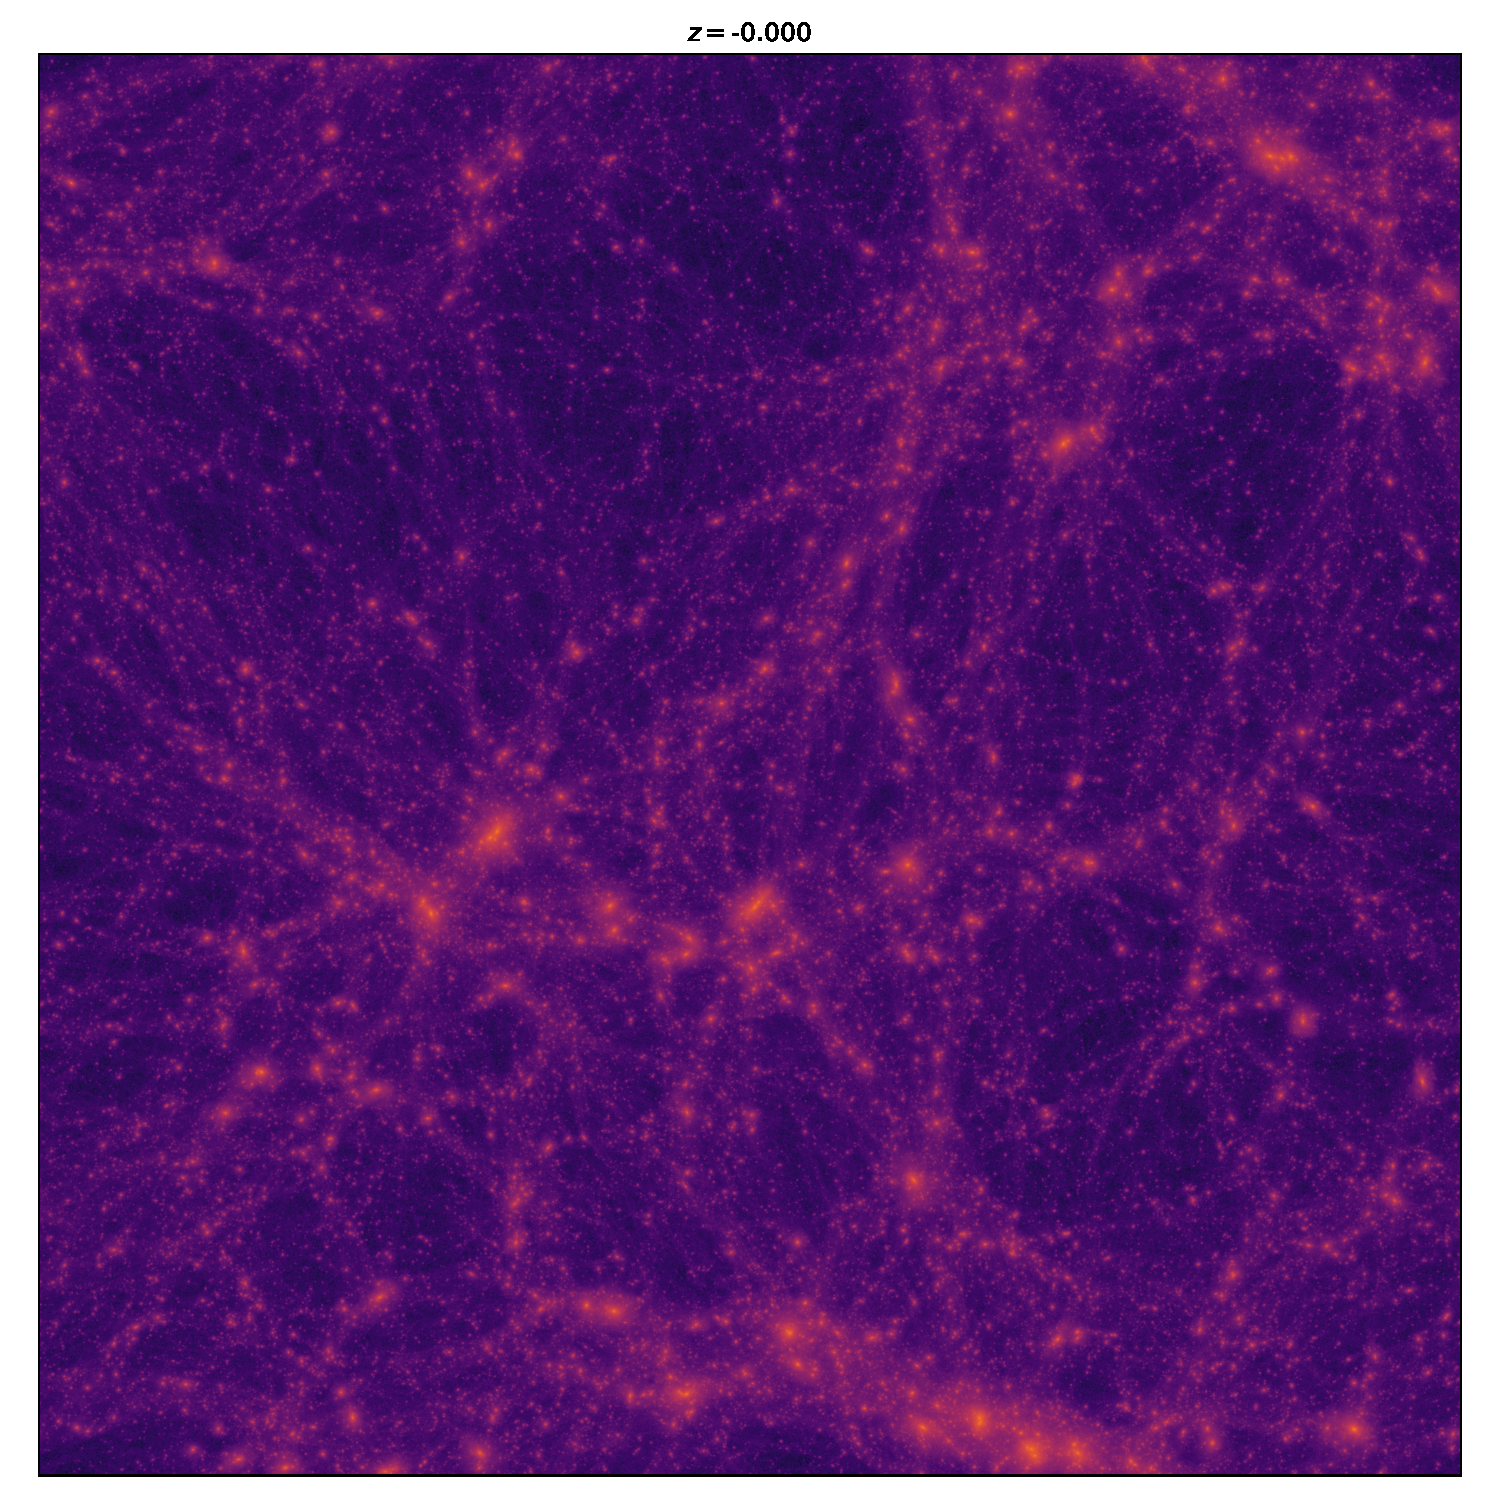
\includegraphics[keepaspectratio,height=\paperheight, width=\paperwidth]{./images/snapshots/particleplot_00041_nolabels.pdf}\hfil}\vfil}}
%    \begin{frame}[plain]
%    \end{frame}
%}

